% T6 of the Transport Papers series.
% Correction (2026-09-10, mechanical pass, per Leon): rule 23 misidentified T5 as the printed-version exception. T1 is the exception at Version 3.0; every other paper, T5 included, reads Version 1.0. \date corrected accordingly (was 1.1).
% v1.1 (2026-09-10, derivation session, Fable 5.1 subagent, per rule 20,
%   series-review repair pass against series_review_2026-09-09.md).
%   Review 2.9: Sec 3 (Prop 3.3 discussion) sentence ending "the complexified
%   Kerr version in Section 6." given its verb: "... inherits unchanged, the
%   scale alone becoming complex" (matches Prop 6.4's "same identity").
%   Review 2.14: Fact 6.10(ii) split. (ii) now imports from Dafermos-Luk only
%   what they prove, the C^0 extension for Kerr perturbations; new (ii') states
%   the generic failure of L^2_loc Christoffels in spherical symmetry with
%   provenance Luk-Oh I/II (new bibitems LukOh2019a, LukOh2019b), and records
%   the Kerr failure as expected/conjectured, not proved. Prop 6.11(2), its
%   proof, Rem 6.12 ("the failed C^1 statement"), and the Sec 1 road map
%   reworded to "proved in spherical symmetry, expected for Kerr". Abstract
%   sentence likewise; to hold the abstract at 250 words "de Sitter or anti-de
%   Sitter" -> "(anti-)de Sitter" and "the strict conformal-over-metric" ->
%   "the conformal-over-metric". Abstract 250 words. \date -> Version 1.1.
%   No label or numbering changed; Fact 6.10 keeps its label and number.
%   Script: verify_T06.py 82/82. Prop 6.2 block now samples the ingoing
%   k = e_t - e_r the prose names, and the outgoing e_t + e_r alongside it,
%   in all four checks; count unchanged.
%   Compile: pdflatex x2, 31 pages, 0 errors, 0 undefined refs, 0 multiply
%   defined, 0 overfull, no float overflow.
%   Addendum 2026-09-09 (coordinator, same review-repair session): the ButlerT7
%   bibitem subtitle brought up to T7's current title ("State, Continuum, Lift,
%   and the Finite-Ledger Seam"). Bibliography only; nothing else changed.
% 2026-09-09 addendum (interactive session with Leon, Opus 5). Two changes
%   per Leon: (1) the printed version is now 1.0 for every paper T0 to T17,
%   T5 alone at 3.0 (progress-doc rule 23); the development numbering is
%   retired from the title page and kept in this header. (2) Every reference
%   to the programme monograph is removed (rule 24), re-pointed to the series
%   where a sibling paper carries the result and otherwise restated to stand
%   alone. No mathematics, no labels and no numbering changed, so verify_T06.py
%   stands unchanged at 82/82 and was not re-run.
%   Here: Remark 4.9 restated as "Convention note on the sign of the norm",
%   giving the convention and why the opposite sign cannot carry the de Sitter
%   stabiliser; the curvature-sign parenthetical dropped. Page count 31 -> 30.
% v1.6 (2026-09-08, derivation session, Fable 5.1 subagent, per rule 20,
%   review-repair pass against T06_review_v13.md).
%   B1: Def 5.5 now imposes the Kasner-type constraint sum p_i^2 = 1 on the
%     admissible class (Schwarzschild satisfies it, Lem 5.1); Thm 5.11's
%     proof bounds ||H|| <= 1 by Cauchy-Schwarz and the constant is
%     exp(lambda(1 + ||E||)) in the statement, the proof and Cor 5.12.
%   B2: the "rates in tau" check reads the leading exponents of tau, delta
%     and epsilon off the constructed series against the tau(r) inversion.
%   S1: Thm 5.6's statement sentence on the phi-lines now points to Thm 5.11
%     and Cor 5.12 and names what remains open (tangential derivatives of E).
%   S2: abstract count updated. S3: epsilon built from the tau series at
%     cot(theta) = 3/4, leading (2/3) cot(theta) r^{1/2} asserted, bracket
%     equals S(r). S4: "nonzero limiting values in the boost part of the Levi
%     factor, which generates it, and zero in the nilradical" at Rem 5.7 and
%     Rem 5.10. S5: Section 5.5 named in Contribution (3), the Proved list
%     (Thm 5.11, Cor 5.12) and the abstract. S6: CONTROL prints an explicit
%     SKIPPED line without numpy/scipy; both counts stated in Section 9 and
%     the script header.
%   N1, N2, N3 (operator norm named, ||1|| = ||B_i|| = ||R_ij|| = 1), N6,
%   N10 (title "What the two ends of the geometry jointly say"), N13, N14
%   (v1.5 block corrected in place: Lem 4.8), N15, N16 (three delta
%   coefficients and the sign of every computed one) done. \date fixed
%   (was 1.2). Checks 81 -> 82: +1 (Def 5.5 / Thm 5.11 Cauchy-Schwarz bound
%   at rational unit directions); B2, S3, N16 replaced in place. Without
%   numpy/scipy: 81 exact, one SKIPPED line.
%   Abstract 249 words raw, 245 stripped. Compile: pdflatex x2, 31 pages,
%   0 errors, 0 undefined, 0 multiply-defined, 0 overfull, no float overflow;
%   numbering frozen: aux diff empty (prop:killing's aux line reorders only
%   because it moved from p.23 to p.24, past the figure). 0 em dashes.
% v1.5 (2026-09-08, prose pass, Fable 5.1 subagent, per project rule 22: mannered
%   prose replaced by literal statement, Leon's ruling to replace the recurring
%   vocabulary too). Body only; no mathematics, numbers, labels or citations
%   changed. About 90 sentences edited, mostly single-phrase replacements.
%   Glossary items applied: "forward ledger" -> "open directions" (1); "the bet"
%   -> "the prediction" (1); "honest limits" -> "limits" (1); "verdict(s)" ->
%   "conclusion(s)" (5, label rem:verdict kept); "machinery" -> "theory/results/
%   calculus" (4); "pins/pinned/sign-pinning" -> "fixes/fixed/sign-fixing" (5,
%   Lem 4.8 title now "The sign is fixed internally", label lem:signpin kept);
%   "lives/sits" -> "lies" (8); "face" -> "instance" (2); "touchpoints" ->
%   "points of contact" (2); "dies" (metric description) -> "fails" (1);
%   "kills" -> "excludes" (1); "paid off" -> "removed" (2); "costs" ->
%   "requires" (1); "bookkeeping" -> "notation/redescription" (2); "picture"
%   -> "computations/case/description" (3); "seed" -> the plain phrase (1).
%   Non-glossary: "silenced/silences/silence" (nilradical) -> "no component in
%   / zero limiting value in / vanishing of the component" (6); "excites" ->
%   "gives nonzero limiting values in" (2); "nilpotent wings" -> "summands" (2);
%   "instalment(s)" -> "half/halves" (7, two section titles); "home ground" ->
%   "the case the framework was built for"; "story" -> "geometry"; "decoration"
%   -> "something added"; "thread/circle closes" -> "argument/structure,
%   completed"; "knits together" -> "connects"; "outlives" -> "persists where
%   ... fails"; "locked" -> "related"; "province of" -> "belongs to".
%   Compile: pdflatex x2, 30 pages, 0 errors, 0 undefined references, 0
%   multiply-defined labels; numbering unchanged (aux diff empty); 0 em
%   dashes; abstract 241 words. verify_T06.py untouched: 81/81, unchanged.
% v1.4 (2026-09-08; derivation session, Fable 5.1, per rule 20: this block is
%   the authoritative record; the mechanical pass does the paperwork). Fold-in
%   of Section 2 of the companion note "Four Programmes, Their Blocks Named"
%   (2026-09-07) per the gap merge plan, T6 entry. NUMBERING FROZEN AND
%   PRESERVED: every pre-existing label keeps its number (checked against the
%   v1.3 .aux, zero changes); the new material is a new subsection at the END
%   of Section 5, so the inbound locators 5.1-5.9 are untouched.
%   NEW subsection 5.5 "Transport along tangential curves, and the phi-lines":
%     Thm 5.11 (Duhamel bound: for every admissible metric, the transport
%       along any tangential curve of fixed Hubble-normalised length converges
%       to the Kasner-model transport, ||T - T^0|| <= lambda ||E_tau||
%       exp(lambda(2 + ||E_tau||)), no weight-by-weight conjugation control);
%     Cor 5.12 (the Schwarzschild phi-lines exactly: generator constant along
%       the line, delta(r) = -(2/15) r - ..., epsilon(r) = (2/3) cot(theta)
%       r^{1/2}(1 + (3/10) r + ...), rate tau^{1/3}; tangential regularity at
%       Schwarzschild by SO(3) x R_t symmetry);
%     Rem 5.13 (what is closed: the transport-level half of the edge problem
%       for the whole admissible class; what remains: tangential derivatives
%       of E_tau in general).
%   Thm 5.6's proof: the phi-line disclaimer now points to Thm 5.11 (one
%     sentence). Successor problem (4) restated to its remaining half; the
%     closing sentence "depends on (2) and (4)" replaced: the nu bet is stated
%     at Schwarzschild where (2) does not arise and (4) is closed, so it waits
%     on the calibration of the count, not on analysis here. T5's conditional
%     steps that cite the old dependence by name are T5's to reword (recorded
%     in the plan, not applied). Machine verification updated.
%   Script verify_T06.py v1.4: new Part (Section 5.5) = the note's Part A,
%     retagged [Cor 5.12]: five exact checks on the series (S(r), tau sigma_3,
%     one-signedness, the r^{1/2} rotation coefficient, the rate exponents)
%     and one CONTROL check in floating point on the transport exponentials
%     (marked; the verification section now says so). 81/81, run in the
%     session's workspace against the suite's GA.py.
%   Compile: pdflatex x3, 30 pages, 0 errors, 0 undefined references, 0
%     overfull boxes; 0 em dashes.
% v1.3 (derivation pass, 2026-08-31, from the re-review of v1.2; same-day
%   follow-up). The re-review confirmed every v1.2 fix, including the global
%   sign flip, and found one regression plus a set of residues. All applied.
%   REGRESSION FIXED: admitting Lambda != 0 into Def 5.5 left Thm 5.6(4)
%   calling so(1,3) the Levi factor of a PARABOLIC stabiliser, which Thm 5.9
%   denies for Lambda > 0 (non-null frozen point, reductive stabiliser, no
%   nilradical). Clause (4) now states the computed algebra as Lambda^2 W and
%   splits the reading by Lambda: Levi factor of the parabolic for Lambda = 0,
%   proper subalgebra of the reductive stabiliser otherwise. The proof says
%   the same and drops the mis-scoped "when Sch = 0" (the sigma- and rho-slots
%   are fed from mu alone whatever the Schouten tensor). Abstract, intro and
%   Contribution item (3) follow; the values-level qualifier added to (3).
%   STATEMENT REPAIRS: intro's conformal prefactor and Prop 3.3's closing
%   sentence carry the new sign (-M/r^3); Prop 6.2(2)'s EF check names the
%   INGOING congruence correctly as k = e_t - e_r (e_t + e_r is outgoing),
%   with the dual and the advanced time printed; Rem 5.8's scope now names
%   what the Einstein class actually contains (Schwarzschild, SdS, vacuum
%   Kasner with p_i != 0) instead of "the type-D interiors", which the
%   Einstein hypothesis excludes for the charged members; Prop 6.11's
%   preamble no longer calls item (2) "proved here outright" (its proof
%   consumes Fact 6.10(ii), so all three are readings with proved translation
%   steps); Thm 4.5's parenthetical says ALMOST Ricci-flat, with the zero set
%   named; Prop 4.3(3)'s two-step nilpotency is now quantified to non-null w
%   (the square vanishes for null w, and the script's loop is over non-null
%   frame vectors); Lem 4.2(i)'s proof no longer invokes the symmetry of Sch,
%   which it does not use; Fact 6.7 and Prop 6.8 no longer read circularly,
%   the Psi_2 clause named as the spinor-calculus face of the computation
%   rather than an input, with the Mfrak-to-Psi_2 identification stated.
%   SCRIPT (55 -> 71 -> 75 checks): the sign convention is now PINNED, which
%   it was not; a flipped Mfrak with matching expectations previously passed
%   all 71. New Prop 6.4(4) check at a = 0 recovers Fact 2.2's numerical
%   eigenvalues +2M/r^3 and -M/r^3 from R = -(M/r^3)S, with the opposite
%   convention as a failing control. Kasner exponents now have one source of
%   truth (KASNER), tied to the computed rate limits, so corrupting them
%   fails two checks instead of none. The R-variable check does real work: the
%   R-expansion is peeled from the rates by exact series division against
%   R(rho), constants read off, residual required to start at rho^6. The disc
%   scale's inverse cube is built independently (zdbar^3/c^6), removing the
%   tautological conjunct. A non-symmetric Schouten sample pins the index
%   order of the tractor connection's sigma slot. Every new or repaired check
%   was mutation-tested and fails when it should. Sec 9's opening sentence no
%   longer claims to verify EVERY identity: it claims Parts one and two plus
%   Part three's printed constants, which is what the script does.
%   SIBLINGS (same pass): T12 cited Thm 4.5, the null-norm theorem, for the
%   norm Lambda/3, now Thms 4.5 and 4.7; T11 cited T6 Sec 2 for the monograph
%   sign flag, which lives in Rem 4.9; T4 put mixmaster INSIDE T6's
%   admissibility class, where T6's integral diverges, and its restatement of
%   Def 5.5 dropped "locally uniformly on the boundary base"; T17's T6 row
%   was two versions stale (25pp/54). Separately, T6 described T5's chain as
%   "ten-step" in the introduction and the Position section: that is the
%   monograph's sequential numbering, which T5 retired (T5 runs T1's SIX-step
%   transport algorithm as Steps 1-3, 4a-4e, 5, 6a-6b, with the dictionary to
%   the old numbering in its own text). Both sites now read six-step. T7 and
%   T17 carry the same stale description and are flagged, not touched here.
%   OPEN, FOR LEON: the rule-17(b) status of the Butler2026 monograph
%   citation (T6 no longer depends on it; it survives as commentary at
%   Prop 3.3's proof and Rem 4.9). T17 also carried three stale prose copies
%   of the series check total (534, 512, 966) contradicting its own audit
%   script; since the T6 row moved that number, all four were reconciled to
%   987 and verify_T17.py's counts/pages dicts updated (T6 54 -> 75,
%   25 -> 28pp). T17 audit back to 37/37.
%   COMPILE: pdflatex x2 clean, 28 pages, no undefined references.
%   verify_T06.py: 75 checks, all pass. Abstract 242 words; 0 em dashes.
% v1.2 (derivation pass, 2026-08-31, from Leon's semantic review of this
%   date; same-day follow-up to v1.1). Four blocking, seven serious, and the
%   minor items, all at the statement layer; the underlying computations
%   stood. BLOCKING: (1) Def 5.5 now requires Einstein (Ric = Lambda g,
%   Lambda constant) alongside E_tau -> 0 and integrability; the class is
%   renamed Einstein velocity-dominated, and Thm 5.6's tractor clauses are
%   proved with Sch = (Lambda/6) g (the reviewer's a_i = tau^(1/2)
%   counterexample shows no decay condition alone can carry them). Abstract,
%   intro, contribution, delimiter, and scope wording follow. Knock-on
%   applied in T4 (Fact 8.25). (2) Prop 6.11(2) restated as the derivative-
%   level filtration (point-level survives, connection-level fails, metric
%   and conformal alike); the conformal-over-metric separation is now
%   explicitly the open transport question; abstract, intro, and Rem 6.12
%   headline sentences rewritten to match. (3) Prop 6.2(2): the display
%   h(a).h(b) is the INVERSE metric; the metric is g = eta - 2H k(x)k by the
%   paper's own g = hinv.hinv, EF-checked at a = 0; statement and proof
%   fixed, script now checks both identities at three H. (4) verify_T06's
%   Killing check rebuilt: Mfrak from an independent inverse cube
%   (zbar^3/|z|^6), plus exponent controls at two and four. SERIOUS:
%   Thm 4.5 scale-anchored (parallelism of I_g, existential form demoted to
%   a parenthetical on the weaker conformally invariant statement);
%   R = -(M/r^3)S throughout (Prop 3.3, Fact 6.3, Prop 6.4), matching
%   Fact 2.2 and T5, convention change now declared in the statement, not a
%   proof; Fact 2.2 provenance corrected (radial from the gauge field,
%   Prop 2.4(1); mixed/angular via Cartan in the static chart, App. A);
%   Thm 5.6's final clause now states the Hubble-normalised t/theta-line
%   comparison and the tau-geodesic log-ratio as separate statements (the
%   fixed-coordinate-segment comparison diverges and is disclaimed);
%   Prop 6.11(1) rerouted through T5 Prop 3.1 + T4 Thm 4.4/Cor 4.5,
%   "generic" dropped; ideal point no longer called the unique off-embedding
%   null ray (light cone at infinity named, n_inf its vertex); Fact 6.7's
%   Psi_2 ~ chi^{-3} clause scoped with internal re-verification named.
%   MINOR: Lem 5.2(3) restricted to diagonal data with the O(tau^{1/3})
%   sphere rate stated; Prop 6.4(3) hypotheses a != 0; Prop 3.1(4) "null"
%   now names the rescaled boundary form; values-level qualifiers in
%   abstract and intro; S^2 patchwise remark in Def 5.5; Figure 1 now
%   referenced from Rem 6.5. Script: trace and p_i checks made live,
%   nilpotency loops all four w with N^2 != 0, wider sampling (beta = 1
%   horizon value included; three H; three t and two x for the translation
%   exponential; three group-law pairs; R-variable composition performed);
%   tractor-connection block added (metric preservation with flipped-sign
%   control, nabla I_g, Einstein parallelism and both norms through the
%   tractor metric, non-Einstein control). T8's Kretschmann provenance
%   repaired in T8 (same pass). Monograph citation at Prop 3.3 kept but the
%   statement made self-standing; the rule-17(b) status of Butler2026 is
%   flagged for Leon's ruling, not resolved here.
%   COMPILE: pdflatex x2 clean, 27 pages, no undefined references.
%   verify_T06.py: 71 checks, all pass. Abstract ~247 words; 0 em dashes.
% v1.1 (derivation pass, 2026-08-31, from Leon's review of this date): rigor
%   and retrofit pass, no result renumbers (checked: verify_crossrefs T06,
%   40/40, inbound and outbound).
%   (1) Def 5.5: admissibility strengthened (E_tau -> 0 added alongside the
%   integrability); the boundary bundle and a values-level boundary holonomy
%   algebra are now defined there, so Thm 5.6(4) computes a defined object.
%   (2) Thm 5.6 restated and reproved at that standard: the Duhamel gloss and
%   the Ambrose-Singer paragraph are gone; holonomy is values-level via
%   Lem 5.4; the exact abelian transport comparison is confined to the t- and
%   theta-lines where it is true; the phi-line noncommutativity (boost beside
%   the tau-independent cos(theta) R_23) is stated, with the transport-level
%   upgrade registered in successor problem (4). Thm 5.9 inherits through the
%   constant-section argument (mu-component zero, annihilated by the values).
%   (3) Prop 4.3(3): the exact translation exponential e^{tN}X(x) = X(x-tw)
%   is now printed in the proof (was deferred to the script) and checked.
%   (4) Lem 5.2(3): "monotone" replaced by proved one-signedness of the
%   deviations (power series in sqrt r, nonzero leading coefficient).
%   (5) Fact 6.7 gains the Psi_2 proportional to chi^{-3} clause with its
%   provenance; Prop 6.8's proof now cites the Fact instead of asserting it.
%   Prop 6.11's preamble states which items are readings of imports.
%   (6) Rules 16c/17/18 retrofit: "Position in the series" added as Sec 8,
%   between Scope and Machine verification, so no theorem or externally
%   cited section renumbers (T8 cites Secs 5 and 7; checked); stale
%   "forthcoming" wording removed in the intro and the T9 remark (which now
%   cites ButlerT9); bibitems added for T0, T7, T8, T9, T10; orphan
%   Penrose2010 bibitem removed; bib key ButlerVerifyT07 renamed
%   ButlerVerifyT06. Version bumped to 1.1 in \date.
%   COMPILE: pdflatex x2 clean, 26 pages, no undefined references.
%   verify_T06.py: 55 checks, all pass (54 + the new translation-exponential
%   check); abstract 244 words; 0 em dashes; disclaimer verbatim.
% 2026-08-24: retitled (was "The Geometry of the Ascent") per Leon; content unchanged.
% v1.0 (sprint 2, 2026-08-21): review draft, M1-M6 complete. M1 skeleton + Sections 1-3 (setup,
% unipotent ray, exact scale decoupling); M2 Section 4 (parallel ideal
% point); M3 Section 5 (Kasner form, weighted limit, SdS).
% House rules: no em dashes; short abstract; standard series disclaimer;
% physics touchpoints kept (rule 10); proof standard per rule 11 (Fact
% (imported) discipline); verification imports GA.py (rule 12); diagrams
% per rule 13.
\documentclass[11pt]{article}
\usepackage[margin=1.1in]{geometry}
\usepackage{amsmath,amssymb,amsthm,mathtools}
\usepackage{booktabs}
\usepackage[dvipsnames]{xcolor}
\usepackage{tikz}
\usepackage[colorlinks=true,linkcolor=MidnightBlue,citecolor=MidnightBlue,urlcolor=MidnightBlue]{hyperref}

\newtheorem{theorem}{Theorem}[section]
\newtheorem{proposition}[theorem]{Proposition}
\newtheorem{lemma}[theorem]{Lemma}
\newtheorem{corollary}[theorem]{Corollary}
\theoremstyle{definition}
\newtheorem{definition}[theorem]{Definition}
\newtheorem{remark}[theorem]{Remark}
\newtheorem{example}[theorem]{Example}
\newtheorem{conjecture}[theorem]{Conjecture}
\newtheorem{fact}[theorem]{Fact}

\newcommand{\Cl}{\mathrm{Cl}}
\newcommand{\R}{\mathbb{R}}
\newcommand{\C}{\mathbb{C}}
\newcommand{\HH}{\mathbb{H}}
\newcommand{\Mat}{\mathrm{M}}
\newcommand{\hb}{\bar{h}}
\newcommand{\er}{e_r}
\newcommand{\et}{e_t}
\newcommand{\Ric}{\mathrm{Ric}}
\newcommand{\Sch}{\mathrm{P}}
\newcommand{\tr}{\operatorname{tr}}
\newcommand{\id}{\mathrm{id}}
\newcommand{\nO}{n_0}
\newcommand{\nInf}{n_\infty}
\newcommand{\ip}[2]{\langle #1, #2\rangle}

\title{\bfseries The Geometry of the Black-Hole Interior\\[4pt]
  \large\itshape Where Division Fails, the Weighted Limit, and the Kerr Tests}
\author{Leon Butler\\ \normalsize\href{mailto:lbutler.math@gmail.com}{\texttt{lbutler.math@gmail.com}}\\ \normalsize ORCID: \href{https://orcid.org/0009-0006-4449-5617}{0009-0006-4449-5617}}
\date{Version 1.0, September 2026 \textperiodcentered{} Transport Papers, T6}

\begin{document}
\maketitle

\begin{abstract}
\normalsize
This paper is the mathematical-relativity companion to T5: the geometry of the ascent $\Cl(1,3) \to \Cl(2,4)$ at the black-hole singularity, in three parts. Part one, where division fails: the Schwarzschild gauge field is a ray in a one-parameter unipotent group, and the curvature factorises exactly, at every radius, into a divergent conformal scale times a fixed shape operator $S$ satisfying $S^2 + S = 2$. Part two, the covariant form: the vacuum field equations are exactly equivalent to the covariant constancy of the null scale section of the rank-six tractor bundle, a parallel ideal point; for $\Lambda \neq 0$ the point leaves the cone with squared norm $\Lambda/3$, and its stabiliser rotates from parabolic Poincar\'e to reductive (anti-)de Sitter. Part three, the approach and the tests: under a blow-up weighted by the Kasner exponents $(-\tfrac13, \tfrac23, \tfrac23)$ the tractor formulation extends to the singular locus for the Einstein velocity-dominated class, with values-level boundary holonomy exactly $\mathfrak{so}(1,3)$, for $\Lambda = 0$ the Levi factor of the frozen point's parabolic stabiliser, and transport-level convergence along tangential curves of fixed Hubble-normalised length; and Kerr passes three tests: unipotency on a null shear, a complex factorisation locating the ring and leaving the disc regular, and the conformal scale as the inverse cube of the Walker-Penrose Killing spinor. At the perturbed Cauchy horizon point-level structure extends continuously while connection-level structure generically fails, proved in spherical symmetry and expected for Kerr; the conformal-over-metric separation is the sharpest open problem. Eighty-two checks verify the computational identities.
\end{abstract}

\medskip
\noindent\textbf{MSC 2020.} Primary 83C57, 53A30; Secondary 15A66, 53C50, 83C20.\\
\textbf{Keywords.} gauge theory gravity; Schwarzschild singularity; tractor calculus; almost-Einstein; Kasner; BKL; weighted blow-up; Kerr; Kerr-Schild; Killing spinor; Cauchy horizon.

\newpage
\textbf{Authorship and disclosure. }The founding idea of the series is the author's: that division by zero in a Clifford algebra should be read not as a prohibition but as a transport into a higher-dimensional algebra, and that the transported division need not be accompanied by an inverse operation. The direction of investigation and the critical review of the results are likewise the author's. The mathematical development and the drafting of the text were carried out in extended collaboration with Claude Fable 5 (Anthropic), an AI system.

\newpage
\section{Introduction}\label{sec:intro}

T5 of this series \cite{ButlerT5} runs a six-step chain from the Schwarzschild gauge field to the Page curve, and at three of its links it defers to a companion geometry paper: for the detailed geometry of where and how division fails, for the covariant meaning of the ascent at the level of the field equations, and for the tests that decide whether the ascended description has physical content or is only a redescription. This is that paper.

The object under study is the gauge-theoretic formulation of general relativity in the spacetime algebra $\Cl(1,3)$, due to Lasenby, Doran and Gull \cite{LDG1998}: gravity as a position-dependent linear map $\hb$ on a flat background, with every metrical statement built from $\hb^{-1}$. The theory's geometric content exists exactly where $\hb$ is invertible, and the series' transport principle \cite{ButlerT1} is a general theory of the loci where it is not. Three questions arise the moment the principle is applied to a black hole, and they organise the paper's three parts.

\emph{Where, exactly, does division fail, and what is the algebraic character of the approach?} Part one (Section \ref{sec:fails}) answers with two exact factorisations. The Schwarzschild gauge trajectory is a ray in a one-parameter unipotent group: at every radius the field is a finite null-type shear of the identity, and the singularity is the divergence of the shear parameter (Proposition \ref{prop:unipotent}). The curvature factorises exactly, at every radius, into a divergent conformal prefactor $-M/r^3$ times a fixed, mass-independent shape operator $S$ satisfying $S^2 + S = 2$ (Proposition \ref{prop:shape}): the entire approach to the singularity is carried by a single conformal weight, and what survives the approach is conformal data.

\emph{Is the ascent $\Cl(1,3) \to \Cl(2,4)$ a property of the equations or something added to them?} Part two (Section \ref{sec:tractor}) proves the strongest available answer: no limit is needed. The vacuum field equations are exactly equivalent, at every radius, to the covariant constancy of the distinguished null scale section of the rank-six ambient (tractor) bundle: a parallel ideal point of the fibre quadric (Theorem \ref{thm:parallel}). The equations of vacuum gravity are natively a statement in the ascended description, and the familiar metric form is what that statement looks like after a scale is chosen. The cosmological constant enters at theorem level: for $\Lambda \neq 0$ the frozen point leaves the cone, its squared norm is $\Lambda/3$, and its stabiliser rotates from the parabolic Poincar\'e group to the reductive de Sitter or anti-de Sitter group (Theorem \ref{thm:lambda}, Proposition \ref{prop:stabiliser}): $\Lambda$ measures precisely the failure of infinity to be parabolic.

\emph{Does the covariant description actually reach the singularity?} Part three answers in two halves. Section \ref{sec:approach} proves the weighted limit theorem: blowing up the interior along the singular locus with direction-dependent weights equal to the Kasner exponents $(-1/3, 2/3, 2/3)$, the Hubble-normalised connection and the parallel tractor extend continuously to the exceptional boundary, with explicit rates ($O(\tau^{2/3})$ in the boosts, $O(\tau^{1/3})$ in the rotations), and the values-level boundary holonomy algebra is exactly $\mathfrak{so}(1,3)$, which for $\Lambda = 0$ is the Levi factor of the frozen point's parabolic stabiliser with no component in the nilradical, and for $\Lambda \neq 0$ a proper subalgebra of its reductive stabiliser (Theorem \ref{thm:weighted}). The theorem is proved in full for the Schwarzschild class, extends verbatim to Schwarzschild-de Sitter (Theorem \ref{thm:sds}), and carries a sharp delimiter: for generic mixmaster singularities the frame limit provably fails to exist, and the correct generic statement must be billiard-invariant (Remark \ref{rem:delimiter}). Section \ref{sec:kerr} then runs the Kerr tests: the whole Kerr family is unipotent on a null shear (Proposition \ref{prop:kerrschild}); the curvature takes the Schwarzschild form with a complexified scale whose non-invertibility locus is exactly the ring, with the disc interior regular (Proposition \ref{prop:ring}); the complex scale is the inverse cube of the Walker-Penrose Killing spinor, so the framework's scalar-plus-pseudoscalar scale is a hidden twistorial object (Proposition \ref{prop:killing}); and at the perturbed Cauchy horizon the imported PDE results establish survival by derivative level, point-level structure (metric and conformal alike) extending continuously while connection-level structure generically fails (proved in spherical symmetry, expected for Kerr), with the strict conformal-over-metric separation registered as the sharpest successor problem (Section \ref{subsec:cauchy}).

\subsection*{Prior art}

Each part of the paper relies on named prior art, and the boundaries are declared here once. \emph{Gauge theory gravity} is due to Lasenby, Doran and Gull \cite{LDG1998}, with the textbook treatment in \cite{DoranLasenby2003}; the field equations, the Newtonian (Painlev\'e-Gullstrand) gauge, and the Kerr-Schild forms used below are theirs, and the curvature computations we import are so marked. \emph{Tractor calculus} goes back to Thomas and was formalised by Bailey, Eastwood and Gover \cite{BEG1994}, with the modern treatment in Curry-Gover \cite{CurryGover2018}; the almost-Einstein characterisation (Einstein metrics as parallel scale tractors) is Gover's \cite{Gover2010}, and Theorem \ref{thm:parallel} is that characterisation put to a new use: the reading of the GTG vacuum equations as the covariant constancy of an ideal point of the series' completion, and the identification of the parabolic stabiliser structure with the obstruction structure of \cite{ButlerT1}, are the contributions claimed, not tractor calculus itself. The \emph{Kasner} form of the Schwarzschild interior is classical (Kantowski-Sachs), and the velocity-dominated class descends from Eardley-Liang-Sachs \cite{ELS1972} and Isenberg-Moncrief \cite{IsenbergMoncrief1990}; BKL oscillations and the billiard description are \cite{BKL1970, DHN2003}; the weighted limit theorem and its holonomy identification are new. On the Kerr side, the Kerr-Schild form is \cite{KerrSchild1965}, the Killing spinor is Walker-Penrose \cite{WalkerPenrose1970} with Carter's constant \cite{Carter1968}; mass inflation is Poisson-Israel \cite{PoissonIsrael1990}, the $C^0$ stability of the Kerr Cauchy horizon with generic curvature blow-up is Dafermos-Luk \cite{DafermosLuk2017}, and the finiteness of tidal distortion is Ori \cite{Ori1991}. What part three adds is the reading: the location of the framework's own criteria inside these results, and the conclusion they jointly support about the ascent.

\subsection*{Contribution}

At the standard of \cite{ButlerT1}, with each theorem carrying its own hypotheses and imports stated as Facts with provenance. (1) The exact algebra of the failure: the unipotent ray and the exact scale decoupling $S^2 + S = 2$ (Section \ref{sec:fails}). (2) The covariant form of the vacuum equations as a parallel ideal point, with a self-contained flat-model dictionary that fixes every sign, the $\Lambda \neq 0$ extension, and the parabolic-to-reductive stabiliser rotation proved outright (Section \ref{sec:tractor}). (3) The weighted limit theorem for the Einstein velocity-dominated class, with explicit Kasner data, explicit convergence rate, the values-level boundary holonomy, the mixmaster delimiter, and the Schwarzschild-de Sitter extension, together with transport-level convergence along every tangential curve of fixed Hubble-normalised length for the whole admissible class and the explicit $\tau^{1/3}$ rate of the Schwarzschild $\varphi$-lines (Section \ref{sec:approach}, Subsection \ref{subsec:tangential}). (4) The Kerr tests: unipotency across the family, the complex factorisation locating the ring, the Killing-spinor identification of the scale, the duality-monodromy conjecture, and the Cauchy-horizon filtration reading of the PDE literature (Section \ref{sec:kerr}). (5) Machine verification of every computational identity in exact arithmetic \cite{ButlerVerifyT06}.

\section{Setting and conventions}\label{sec:setting}

Spacetime algebra $\Cl(1,3)$ with orthonormal generators $\gamma_0, \gamma_1, \gamma_2, \gamma_3$, $\gamma_0^2 = +1$, $\gamma_i^2 = -1$; in the $(t,r)$ plane write $\et := \gamma_0$, $\er := \gamma_1$. The pseudoscalar is $I := \gamma_0\gamma_1\gamma_2\gamma_3$, with $I^2 = -1$; $I$ commutes with every even element and anticommutes with every vector. Units $G = c = 1$; metric signature $(+,-,-,-)$. Curvature conventions are those fixed by the Cartan structure equations exactly as in T5's appendix \cite[App.~A]{ButlerT5}; in these conventions the de Sitter metric has $\Ric_{ab} = \Lambda\, g_{ab}$ and scalar curvature $R = 4\Lambda$.

In gauge theory gravity, gravity is a pair of gauge fields on the flat background: the position-dependent linear map $\hb(a)$ on vectors, gauging local frame rescalings, and the connection bivector $\Omega(a)$, gauging local Lorentz rotations. The covariant derivative and field strength are
\[
D_a M = a \cdot \nabla M + \Omega(a) \times M, \qquad
R(a \wedge b) = a\cdot\nabla\,\Omega(b) - b\cdot\nabla\,\Omega(a) + \Omega(a) \times \Omega(b),
\]
with $A \times B := \tfrac12(AB - BA)$, and the field equations are $R(a) - \tfrac12 a R = \kappa\, T(a)$ together with the vanishing of torsion, which determines $\Omega$ algebraically from $\hb$; the metric is $g(a,b) = \hb^{-1}(a) \cdot \hb^{-1}(b)$ \cite{LDG1998}. Every operation in these displays is interior to $\Cl(1,3)$: nothing invokes a curved manifold beyond the flat background. The theory is a field theory of an invertibility-demanding map, which is exactly the condition the transport principle addresses.

\begin{fact}[Imported: equivalence with the Einstein equations]\label{fact:gtg}
On any region where $\hb$ is invertible, the GTG field equations for $(\hb, \Omega)$ are equivalent to the Einstein field equations for the metric $g(a,b) = \hb^{-1}(a)\cdot\hb^{-1}(b)$; in vacuum, to Ricci-flatness of $g$. \emph{Provenance:} Lasenby, Doran and Gull \cite[\S 7]{LDG1998}; textbook form \cite[Ch.~13-14]{DoranLasenby2003}.
\end{fact}

\begin{fact}[Imported: the Schwarzschild curvature spectrum]\label{fact:spectrum}
For the static spherically symmetric vacuum metric $f\,dt_s^2 - f^{-1}dr^2 - r^2 d\Omega^2$ with $f = 1 - 2M/r$, the curvature operator on bivectors is diagonal on the coordinate planes of the orthonormal frame, with eigenvalue of one magnitude, $2M/r^3$, on the radial boost plane $\sigma_r$ and its Hodge dual $I\sigma_r$, and eigenvalue of half that magnitude and opposite sign, $-M/r^3$, on the four mixed planes. \emph{Provenance:} the radial-plane eigenvalue from the gauge field alone in \cite[Prop.~2.4(1)]{ButlerT5}; the mixed- and angular-plane eigenvalues by the Cartan structure equations in the static chart in \cite[App.~A]{ButlerT5}, the two computations agreeing on the invertible region by Fact \ref{fact:gtg}; the same computation in the GTG literature is \cite[Ch.~14]{DoranLasenby2003}.
\end{fact}

These are the only geometric imports of Part one; everything else in Sections \ref{sec:fails} through \ref{sec:approach} is proved here.

\section{Part one: where division fails}\label{sec:fails}

\subsection{The unipotent ray}\label{subsec:unipotent}

For Schwarzschild in the Newtonian (Painlev\'e-Gullstrand) gauge the gauge field is
\begin{equation}\label{eq:hbar}
\hb \;=\; 1 - \beta\,P, \qquad \beta(r) = \sqrt{2M/r}, \qquad P(a) := (a \cdot \et)\,\er .
\end{equation}

\begin{proposition}[The gauge trajectory is a unipotent ray]\label{prop:unipotent}
The map $P$ is nilpotent, $P^2 = 0$, exactly and at every radius. Consequently:
\begin{enumerate}
\item the maps $\{1 + sP : s \in \R\}$ form a one-parameter unipotent group, $(1 + sP)(1 + s'P) = 1 + (s + s')P$, and the entire history of the gauge field, from spatial infinity to the singularity, is the ray $s = -\beta(r) \in (-\infty, 0]$ in this group;
\item $\hb$ is invertible at every $r > 0$ in closed form, $\hb^{-1} = 1 + \beta P$, the horizon $\beta = 1$ included: the horizon is algebraically unremarkable;
\item the metric $g(a,b) = \hb^{-1}(a)\cdot\hb^{-1}(b)$ is the Painlev\'e-Gullstrand line element: $g(\et,\et) = 1 - \beta^2 = 1 - 2M/r$, $g(\et,\er) = -\beta$, $g(\er,\er) = -1$, angular directions untouched;
\item the singularity is the divergence $s \to -\infty$ of the shear parameter: division fails nowhere at $r > 0$ and unavoidably at $r = 0$, where the light cones of $g$ fold onto the single null direction of the kernel, a type-N degeneration \cite[Props.~2.4-2.6, 3.1]{ButlerT5}.
\end{enumerate}
\end{proposition}

\begin{proof}
Nilpotency: $P^2(a) = P\bigl((a\cdot\et)\er\bigr) = (a\cdot\et)(\er\cdot\et)\,\er = 0$, since $\er \cdot \et = 0$. The group law is bilinearity plus $P^2 = 0$: $(1 + sP)(1 + s'P) = 1 + (s + s')P + ss'P^2$. Inversion is the case $s' = -s$. The metric: $\hb^{-1}(\et) = \et + \beta(\et\cdot\et)\er = \et + \beta\er$, and $\hb^{-1}(\er) = \er$ since $\er \cdot \et = 0$; then $g(\et,\et) = (\et + \beta\er)^2 = \et^2 + \beta^2\er^2 = 1 - \beta^2$ (the cross terms cancel by anticommutation of orthogonal vectors), $g(\et,\er) = (\et + \beta\er)\cdot\er = \beta\,\er^2 = -\beta$, and $g(\er,\er) = -1$; the angular generators are untouched by $P$. For (4): the folding computation is short enough to repeat. The null directions of $g$ in the $(t,r)$ plane are the $a = \et + \lambda\er$ with $0 = g(a,a) = 1 - \beta^2 - 2\lambda\beta - \lambda^2 \cdot 1 \cdot (-1)(-1)$; explicitly $g(a,a) = (1-\beta^2) - 2\lambda\beta - \lambda^2$, whose roots are $\lambda = -\beta \pm 1$. As $r \to 0$, $\beta \to \infty$ and both normalised null directions $\tfrac{1}{-\beta\pm1}\et + \er \to \er$: the cone collapses onto the single direction $\er$, the kernel direction, null for the rescaled boundary form in which the collapse is measured \cite[Prop.~2.6]{ButlerT5} (for $g$ itself $\er$ has norm $-1$ at every $r > 0$). That the resulting obstruction is type N and forces Rule 1, and that no gauge choice removes it, is T5's Steps 1-2 \cite{ButlerT5}, quoted here rather than reproved.
\end{proof}

\begin{remark}[Parabolic for a structural reason]\label{rem:parabolic}
The structural family is the one that recurs throughout the series. Unipotent, null-direction-shearing maps are exactly what obstructed the element-level completion in the no-go theorem of \cite[Thm.~4.2]{ButlerT1}: the stabiliser of a null direction contains parabolic null rotations, and their fixed-point-free shear excludes every candidate partner. Proposition \ref{prop:unipotent} says the dynamical approach to the singularity proceeds along a parabolic orbit in the gauge group: the gauge field is, at every radius, a finite null-type shear of the identity, and the singularity is the divergence of the shear parameter. The obstruction of the kinematic theory and the trajectory of the dynamical solution belong to the same conjugacy structure. In Section \ref{sec:approach} this observation is promoted to a theorem: the boundary holonomy of the weighted limit is exactly the Levi factor of the parabolic, with no component in the shearing nilradical.
\end{remark}

\subsection{Exact scale decoupling}\label{subsec:shape}

Write $\sigma_r := \er\et$ for the unit radial spacetime bivector, so $\sigma_r^2 = \er\et\er\et = -\er^2\et^2 = +1$, and let $\Pi$ denote the projection of the six-dimensional bivector space onto the plane pair $\operatorname{span}\{\sigma_r, I\sigma_r\}$.

\begin{proposition}[Exact scale decoupling]\label{prop:shape}
In the conventions of Fact \ref{fact:spectrum}, the Schwarzschild curvature operator is, exactly and at every radius,
\[
R(B) \;=\; -\,\frac{M}{r^3}\,S(B), \qquad
S \;:=\; 1 - 3\Pi \;=\; -\tfrac12\bigl(B \mapsto B + 3\,\sigma_r B \sigma_r\bigr),
\]
where the shape operator $S$ satisfies the algebraic identity
\[
S^2 + S = 2 ,
\]
has spectrum $(-2, -2, 1, 1, 1, 1)$, and is trace-free. The factorisation is exact: $S$ depends on neither $M$ nor $r$, and the entire approach to the singularity changes only the conformal prefactor $-M/r^3$.
\end{proposition}

\begin{proof}
First the algebra of conjugation by $\sigma_r$. For $B$ in the plane pair: $\sigma_r\,\sigma_r\,\sigma_r = \sigma_r$ since $\sigma_r^2 = 1$; and $\sigma_r (I\sigma_r)\sigma_r = I\,\sigma_r^3 = I\sigma_r$ since $I$ commutes with even elements. For each of the four mixed planes, $B$ anticommutes with $\sigma_r$: writing $B = \gamma_a\gamma_b$ with exactly one index in $\{0,1\}$, the product $\sigma_r B$ reorders by two transpositions against one shared and one distinct generator, producing a net sign $-1$, so $\sigma_r B = -B\sigma_r$ and $\sigma_r B \sigma_r = -B\sigma_r^2 = -B$. Hence $-\tfrac12(B + 3\sigma_r B\sigma_r)$ equals $-2B$ on the plane pair and $+B$ on the mixed planes, which is $1 - 3\Pi$. Fact \ref{fact:spectrum} says the curvature is diagonal on exactly these planes with eigenvalues $2M/r^3$ (doubled magnitude, on the pair) and $-M/r^3$ (mixed); since $1 - 3\Pi$ has eigenvalues $-2$ on the pair and $+1$ on the mixed planes, the operator with those eigenvalues is exactly $-\tfrac{M}{r^3}(1 - 3\Pi)$: so $R = -(M/r^3)S$ in the conventions of Fact \ref{fact:spectrum}, fixed once in Section \ref{sec:setting}; only the eigenvalue ratio $2 : (-1)$ and the identity of the distinguished plane pair enter any later argument, and both are convention-free. The identity: $S^2 = (1 - 3\Pi)^2 = 1 - 6\Pi + 9\Pi^2 = 1 + 3\Pi$ since $\Pi^2 = \Pi$, so $S^2 + S = 2$. Spectrum and trace: eigenvalue $1 - 3 = -2$ on the two-dimensional range of $\Pi$ and $+1$ on its four-dimensional kernel; trace $= 4 - 4 = 0$.
\end{proof}

\begin{remark}[Three readings]\label{rem:threereadings}
First, the trace-free curvature is pure Weyl, as vacuum requires, and the Weyl part is precisely the conformally covariant part of curvature: what survives the approach is conformal data. Second, dilations emerge exactly, not asymptotically: normalise by the conformal prefactor and nothing along the trajectory changes at all, a rigidity peculiar to the type-D family and stronger than any generic BKL statement. Third, the spectrum exhibits the classic $2{:}1$ Coulombic tidal structure, stretching along the radial plane at twice the rate of the transverse compression; the ratio is an eigenvalue ratio of $S$, hence a conformal invariant of the approach. The singularity is approached with a fixed, scale-free curvature shape, and the divergence is carried entirely by a single conformal weight. The identity $S^2 + S = 2$, equivalently $(S-1)(S+2) = 0$, is the minimal-polynomial statement of this rigidity, and it is the algebraic identity that the complexified Kerr version in Section \ref{sec:kerr} inherits unchanged, the scale alone becoming complex.
\end{remark}

% === Section 4 (M2): the parallel ideal point ===
\section{Part two: the vacuum equations as a parallel ideal point}\label{sec:tractor}

Part one located the failure of division and the conformal rigidity of the approach. This part proves that the ascent $\Cl(1,3) \to \Cl(2,4)$ is not an operation applied to the field equations from outside: the vacuum equations \emph{are}, exactly and at every radius, a single covariant statement about the rank-six ambient bundle whose fibre algebra is $\Cl(2,4)$. No limit is taken anywhere in this section.

\subsection{The tractor bundle in a scale}\label{subsec:tractorsetup}

Let $M^\circ$ be a region where $\hb$ is invertible, $g$ the physical metric there, and $[g]$ its conformal class. The completion of the series assigns to $[g]$ the ambient (tractor) bundle: the rank-six vector bundle $\mathcal{T}$ which, in the chosen scale $g$, splits as
\[
\mathcal{T} \;\cong\; \R \,\oplus\, TM^\circ \,\oplus\, \R, \qquad \text{sections } (\sigma, \mu^b, \rho),
\]
carrying the tractor metric
\begin{equation}\label{eq:tractormetric}
\ip{(\sigma,\mu,\rho)}{(\sigma,\mu,\rho)} \;=\; g(\mu,\mu) \,+\, 2\sigma\rho .
\end{equation}
With $g$ of signature $(1,3)$ the form \eqref{eq:tractormetric} has signature $(2,4)$: the $\mu$ block contributes $(1,3)$ and the hyperbolic $\sigma\rho$ pairing contributes $(1,1)$. The fibre Clifford algebra is $\Cl(2,4)$ and the structure algebra of the bundle is $\mathfrak{so}(2,4)$, acting through the bivectors of $\Cl(2,4)$: this is the same completion that Rule 1 forces at the degenerate locus \cite{ButlerT1, ButlerT4}, here assembled over the regular region.

\begin{fact}[Imported: the tractor connection]\label{fact:tractor}
The bundle $\mathcal{T}$ carries a canonical connection depending only on the conformal class $[g]$, preserving the metric \eqref{eq:tractormetric}, whose expression in the scale $g$ is
\begin{equation}\label{eq:tractorconn}
\nabla_a(\sigma, \mu_b, \rho) \;=\; \bigl(\nabla_a\sigma - \mu_a,\;\; \nabla_a\mu_b + g_{ab}\,\rho - \Sch_{ab}\,\sigma,\;\; \nabla_a\rho + \Sch_a{}^{b}\mu_b\bigr),
\end{equation}
where $\Sch_{ab}$ is the Schouten tensor of $g$, in four dimensions $\Sch_{ab} = \tfrac12\bigl(\Ric_{ab} - \tfrac{R}{6}\,g_{ab}\bigr)$. \emph{Provenance:} Bailey-Eastwood-Gover \cite{BEG1994}; Curry-Gover \cite[\S 5]{CurryGover2018}. The display \eqref{eq:tractorconn} is their connection written in the curvature conventions of Section \ref{sec:setting}; the relative sign of the Schouten slots against those references is convention-dependent, and Lemma \ref{lem:signpin} fixes it internally, so that no sign in this paper rests on a translation between conventions.
\end{fact}

Two elementary properties we use are proved rather than cited.

\begin{lemma}[Metric parallelism, and the trace of the Schouten condition]\label{lem:elementary}
(i) The connection \eqref{eq:tractorconn} preserves the tractor metric \eqref{eq:tractormetric}. (ii) If $\Sch_{ab} = c\, g_{ab}$ for a function $c$, then $c = \tfrac{R}{24}$ and $\Ric_{ab} = \tfrac{R}{4} g_{ab}$; in particular $\Sch_{ab} = 0$ if and only if $\Ric_{ab} = 0$.
\end{lemma}

\begin{proof}
(i) Along any direction $a$, with primes denoting the slots of \eqref{eq:tractorconn},
\[
\tfrac12\,\partial_a \ip{T}{T} \;=\; \sigma'\rho + \rho'\sigma + \mu^b\mu'_b
= (\nabla_a\sigma - \mu_a)\rho + (\nabla_a\rho + \Sch_a{}^b\mu_b)\sigma + \mu^b(\nabla_a\mu_b + g_{ab}\rho - \Sch_{ab}\sigma).
\]
The genuine derivative terms assemble to $\tfrac12\partial_a(2\sigma\rho + |\mu|^2)$; the remainder is $-\mu_a\rho + \mu_a \rho + \Sch_a{}^b\mu_b\sigma - \Sch_{ab}\mu^b\sigma = 0$, the two Schouten terms being one contraction written with the index raised on either side, so that no symmetry of $\Sch$ is needed.
(ii) Tracing $\Sch_{ab} = c\,g_{ab}$ gives $4c = \tfrac12(R - \tfrac{4R}{6}) = \tfrac{R}{6}$, so $c = \tfrac{R}{24}$; substituting back, $\Ric_{ab} = \tfrac{R}{6}g_{ab} + 2c\,g_{ab} = \tfrac{R}{4}g_{ab}$. If $c = 0$ then $R = 24c = 0$ and hence $\Ric = 0$; the converse is immediate.
\end{proof}

\subsection{The flat-model dictionary}\label{subsec:flatmodel}

The interpretive content of the theorems below lies in the flat model, so we set it out completely; every statement here is proved, and the verification script checks each numerically in exact arithmetic. Let $V := \R^{2,4}$ with a quadratic form of signature $(2,4)$ written, in a scale, as $Q(\sigma,\mu,\rho) = \eta(\mu,\mu) + 2\sigma\rho$ with $\eta$ the Minkowski form. Points of conformal Minkowski space are null rays of $V$: the embedding is
\begin{equation}\label{eq:flatembed}
X(x) \;=\; \bigl(1,\; x,\; -\tfrac12\,\eta(x,x)\bigr), \qquad
\ip{X(x)}{X(y)} = -\tfrac12\,\eta(x - y,\, x - y),
\end{equation}
so $X(x)$ is null for every $x$ and the form recovers the flat conformal structure; the ideal point (``infinity'') is the null ray $\nInf := (0, 0, 1)$: the null rays with $\sigma \neq 0$ are exactly the points \eqref{eq:flatembed}, while $\{\sigma = 0,\ \eta(\mu,\mu) = 0\}$ is the light cone at infinity, a further three-parameter family of null rays, and $\nInf$ is its vertex: the unique null ray with $\sigma = 0$ and vanishing $\mu$-component. For a bivector $u \wedge v \in \Lambda^2 V \cong \mathfrak{so}(2,4)$ the action on vectors is
\begin{equation}\label{eq:bivectoraction}
(u \wedge v)(w) \;=\; \ip{v}{w}\,u - \ip{u}{w}\,v ,
\end{equation}
which is the commutator action $\tfrac12[u\wedge v,\, w]$ of the corresponding bivector of $\Cl(2,4)$ under the identification of $\Lambda^2 V$ with the bivectors.

\begin{proposition}[Stabilisers in the flat model]\label{prop:flatstab}
Fix the null vector $\nInf$ and a second null vector $\nO := (1,0,0)$ with $\ip{\nInf}{\nO} = 1$, and let $W := \{\nInf, \nO\}^\perp \cong \R^{1,3}$. Decompose $\Lambda^2 V = \R\,(\nInf \wedge \nO) \oplus \Lambda^2 W \oplus (\nInf \wedge W) \oplus (\nO \wedge W)$. Then:
\begin{enumerate}
\item the stabiliser subalgebra of the vector $\nInf$ is $\Lambda^2 W \oplus (\nInf \wedge W) \cong \mathfrak{so}(1,3) \ltimes \R^4$, the Poincar\'e algebra, of dimension $10$;
\item the stabiliser subalgebra of the ray $\R^+\nInf$ adds the grading element $\nInf \wedge \nO$ and is the $11$-dimensional maximal parabolic $\mathfrak{p} = (\mathfrak{so}(1,3) \oplus \R) \ltimes \R^4$;
\item the nilradical $\nInf \wedge W$ acts on the point space \eqref{eq:flatembed} as the translations, and on $V$ by null shears: for $w \in W$, $(\nInf \wedge w)^2(V) \subseteq \R\,\nInf$ and $(\nInf \wedge w)^3 = 0$, the nilpotency being two-step exactly for non-null $w$ and one-step for null $w$, since $(\nInf \wedge w)^2(v) = -\ip{\nInf}{v}\,\ip{w}{w}\,\nInf$. These are precisely the transvections that obstruct the element-level completion in \cite[Thm.~4.2]{ButlerT1}.
\end{enumerate}
\end{proposition}

\begin{proof}
Apply \eqref{eq:bivectoraction} to $\nInf$ term by term. $(\nInf \wedge \nO)(\nInf) = \ip{\nO}{\nInf}\nInf - \ip{\nInf}{\nInf}\nO = \nInf \neq 0$: the grading element scales $\nInf$ and so stabilises the ray but not the vector. For $C \in \Lambda^2 W$: both pairings of $\nInf$ against $W$ vanish, so $C(\nInf) = 0$. For $w \in W$: $(\nInf \wedge w)(\nInf) = \ip{w}{\nInf}\nInf - \ip{\nInf}{\nInf}w = 0$, while $(\nO \wedge w)(\nInf) = \ip{w}{\nInf}\nO - \ip{\nO}{\nInf}w = -w \neq 0$. Summing dimensions: $6 + 4 = 10$ for the vector, $11$ for the ray; the Levi decomposition is read off the direct sum. For (3): on a point tractor, $(\nInf \wedge w)\bigl(X(x)\bigr) = \ip{w}{X(x)}\,\nInf - \ip{\nInf}{X(x)}\,w$; here $\ip{\nInf}{X(x)} = 1$ (the pairing of $(0,0,1)$ with $(1, x, -x^2/2)$ through the hyperbolic slot) and $\ip{w}{X(x)} = \eta(w, x)$, so with $N := \nInf \wedge w$ acting on the point tractor: $N(X(x)) = \eta(w, x)\,\nInf - w$, then $N^2(X(x)) = -\eta(w,w)\,\nInf$ (using $N(\nInf) = 0$ and $N(w) = \eta(w,w)\,\nInf$) and $N^3(X(x)) = 0$, so the exponential terminates exactly:
\[
e^{tN} X(x) \;=\; \bigl(1,\; x - tw,\; -\tfrac12\eta(x,x) + t\,\eta(w,x) - \tfrac{t^2}{2}\eta(w,w)\bigr) \;=\; X(x - tw),
\]
the last slot being the completed square $-\tfrac12\eta(x - tw,\, x - tw)$: the flow is exactly the translation flow of the point space, with no projective factor, and the verification script confirms the identity at rational samples. Nilpotency: the image of $(\nInf \wedge w)$ lies in $\operatorname{span}(\nInf, w)$, the image of that span lies in $\R \nInf$ (since $(\nInf\wedge w)(w) = \ip{w}{w}\nInf$ and $(\nInf\wedge w)(\nInf) = 0$), and $\nInf$ is annihilated. The identification with the transvections of \cite{ButlerT1} is the statement that both are the maps $1 + \nInf \wedge w$ fixing the null vector $\nInf$ and shearing its orthogonal complement into it.
\end{proof}

\begin{proposition}[Non-null stabilisers, and the section they act on]\label{prop:flatstabnn}
Let $I \in V$ with $\ip{I}{I} \neq 0$. Then:
\begin{enumerate}
\item the stabiliser subalgebra of $I$ is $\Lambda^2(I^\perp) \cong \mathfrak{so}(I^\perp)$, reductive, of dimension $10$, with trivial nilradical: $\mathfrak{so}(1,4)$ if $\ip{I}{I} > 0$ and $\mathfrak{so}(2,3)$ if $\ip{I}{I} < 0$;
\item the hyperplane section $M_I := \{X \in V : \ip{X}{X} = 0,\ \ip{X}{I} = 1\}$ is, under $Y := X - I/\ip{I}{I}$, the pseudosphere $\{Y \in I^\perp : \ip{Y}{Y} = -1/\ip{I}{I}\}$, a complete constant-curvature Lorentzian $4$-manifold on which the stabiliser acts as the isometry group: de Sitter space for $\ip{I}{I} > 0$, anti-de Sitter space for $\ip{I}{I} < 0$;
\item the polar hypersurface $\{\ip{X}{I} = 0\}$ meets the quadric in the projectivised null cone of $I^\perp$: for $\ip{I}{I} > 0$ a spacelike conformal infinity ($S^3$ with its standard conformal structure), for $\ip{I}{I} < 0$ a timelike one.
\end{enumerate}
\end{proposition}

\begin{proof}
(1) Write $B = I \wedge u + C$ with $u \in I^\perp$ and $C \in \Lambda^2(I^\perp)$, which is possible and unique since $\ip{I}{I} \neq 0$ splits $V = \R I \oplus I^\perp$. Then $B(I) = \ip{u}{I}I - \ip{I}{I}u + 0 = -\ip{I}{I}\,u$, which vanishes iff $u = 0$. So the stabiliser is $\Lambda^2(I^\perp)$, and $I^\perp$ carries the restricted form: signature $(1,4)$ if $I$ is a plus direction, $(2,3)$ if a minus direction. Triviality of the nilradical is the reductivity of orthogonal algebras of nondegenerate forms. (2) For $X \in M_I$: $\ip{Y}{I} = \ip{X}{I} - 1 = 0$ and $\ip{Y}{Y} = \ip{X}{X} - 2\ip{X}{I}/\ip{I}{I} + 1/\ip{I}{I} = -1/\ip{I}{I}$. The map is an affine bijection commuting with the stabiliser. If $\ip{I}{I} > 0$: $I^\perp \cong \R^{1,4}$ and the locus $\ip{Y}{Y} = -1/\ip{I}{I} < 0$ is the standard de Sitter hyperboloid, with induced signature $(1,3)$ and isometry group $O(1,4)$. If $\ip{I}{I} < 0$: $I^\perp \cong \R^{2,3}$ and the locus $\ip{Y}{Y} > 0$ is the standard anti-de Sitter hyperboloid with isometry group $O(2,3)$. (3) Null rays of $I^\perp$: for $\R^{1,4}$ with form $t^2 - \sum_1^4 x_i^2$, the null cone is $t^2 = |x|^2$, whose rays are parametrised by the unit sphere $S^3 = \{|x| = 1, t = 1\}$; the induced degenerate form on the cone descends to a negative-definite form on the ray space, i.e.\ a spacelike (Riemannian) conformal $3$-sphere, the conformal infinity of de Sitter space. For $\R^{2,3}$ the same construction yields ray space $S^1 \times S^2$ (up to cover) carrying a Lorentzian conformal structure: the timelike infinity of anti-de Sitter space.
\end{proof}

\subsection{The vacuum theorem}\label{subsec:vacuumthm}

\begin{theorem}[Covariant form of the vacuum equations]\label{thm:parallel}
Let $g$ be the physical metric on $M^\circ$ and let $I_g := (1, 0, 0)$ be the pure-scale section of $\mathcal{T}$ in the scale $g$. Then
\[
\nabla_a I_g = \bigl(0,\; -\Sch_{ab},\; 0\bigr),
\]
so $I_g$ is parallel if and only if $\Sch = 0$, if and only if $g$ is Ricci-flat, if and only if (Fact \ref{fact:gtg}) the GTG vacuum field equations hold. Moreover $\ip{I_g}{I_g} = 0$: the section is null. Hence the vacuum field equations on $M^\circ$ are exactly equivalent to the parallelism of the scale tractor $I_g$ attached to $g$: the ideal point of the fibre quadric that the physical scale distinguishes is covariantly constant. (Existence of \emph{some} parallel null tractor is the strictly weaker, conformally invariant statement that $[g]$ is almost Ricci-flat: it carries an almost-Einstein scale which is Ricci-flat away from that scale's zero set, and the zero set may be non-empty. A non-constant rescaling $e^{2\omega}g$ already keeps the parallel section while losing the field equations.) The statement is covariant under the gauge transformations of $\mathcal{T}$, whose structure algebra is $\mathfrak{so}(2,4)$ acting through the bivectors of $\Cl(2,4)$.
\end{theorem}

\begin{proof}
Substitute $(\sigma, \mu, \rho) = (1, 0, 0)$ into \eqref{eq:tractorconn}: the first slot is $\nabla_a 1 - 0 = 0$; the second is $0 + g_{ab}\cdot 0 - \Sch_{ab}\cdot 1 = -\Sch_{ab}$; the third is $0 + \Sch_a{}^b \cdot 0 = 0$. So $\nabla I_g = 0$ iff $\Sch_{ab} = 0$ iff $\Ric = 0$ by Lemma \ref{lem:elementary}(ii), and Fact \ref{fact:gtg} converts Ricci-flatness into the GTG field equations on the region of invertibility. The norm is $\ip{I_g}{I_g} = g(0,0) + 2 \cdot 1 \cdot 0 = 0$. Covariance is the statement that both sides of the equivalence are conditions on a section of an invariantly defined bundle with its canonical connection (Fact \ref{fact:tractor}), the section itself determined by the given scale $g$: the splitting used to write the proof is scale-dependent; the bundle, the connection, and the parallelism condition on the given section are not.
\end{proof}

\begin{remark}[What the equation now says]\label{rem:interpret}
In the flat model the parallel null tractor is the ideal point $\nInf$ of Proposition \ref{prop:flatstab}: the point at infinity. Theorem \ref{thm:parallel} therefore reads: \emph{the field equation of vacuum gravity literally asserts the covariant constancy of a distinguished point at infinity}. This is a statement not about metric components but about a preferred ideal point of the fibre quadric, parallel-transported without change over the whole of $M^\circ$. The space it lies in, the point space of the completion, is precisely where \cite[Thm.~4.10]{ButlerT1} located the resolution of division by zero, and precisely the structure that the no-go theorem showed cannot be replaced by any element-level classical assignment. The ascent is not notation added to the physics: the physics, in vacuum, is an assertion within the ascended description, and the familiar metric form of the equations is what that assertion looks like after a scale is chosen. The points of contact with established physics, kept in view as the series' practice requires: the bundle $\mathcal{T}$ is the standard conformal tractor bundle (Thomas; Bailey-Eastwood-Gover), the equivalence ``Einstein $\Leftrightarrow$ parallel scale tractor'' is the almost-Einstein characterisation of Gover \cite{Gover2010}, and the spinor module of the fibre algebra $\Cl(2,4)$ is Penrose's twistor space, whose development belongs to the series' twistor paper.
\end{remark}

\subsection{The cosmological constant: the frozen point leaves the cone}\label{subsec:lambda}

\begin{theorem}[$\Lambda \neq 0$: the scale tractor leaves the cone]\label{thm:lambda}
Let $g$ satisfy the Einstein condition $\Ric_{ab} = \Lambda\, g_{ab}$ on $M^\circ$, in the conventions of Section \ref{sec:setting}, and set
\[
I_g \;:=\; \Bigl(1,\; 0,\; \tfrac{\Lambda}{6}\Bigr)
\]
in the scale $g$. Then $I_g$ is parallel, and every parallel section of the form $(1, 0, \rho)$ arises this way: $(1,0,\rho)$ is parallel if and only if $\rho$ is constant and $g$ is Einstein with $\Lambda = 6\rho$. The norm is
\[
\ip{I_g}{I_g} \;=\; \tfrac{\Lambda}{3} :
\]
the frozen point is null exactly in the $\Lambda = 0$ vacuum, and for $\Lambda \neq 0$ it leaves the cone, with the cosmological constant as its squared norm (times the positive constant $3$).
\end{theorem}

\begin{proof}
Substitute $(1, 0, \rho)$ into \eqref{eq:tractorconn}: the slots are $(\,-0,\; g_{ab}\rho - \Sch_{ab},\; \nabla_a \rho\,)$. Parallelism therefore requires $\rho$ constant and $\Sch_{ab} = \rho\, g_{ab}$; by Lemma \ref{lem:elementary}(ii) this forces $\Ric_{ab} = \tfrac{R}{4}g_{ab}$ with $\rho = \tfrac{R}{24}$, i.e.\ the Einstein condition with $\Lambda = \tfrac{R}{4} = 6\rho$. Conversely, for Einstein $g$ with $\Ric = \Lambda g$: $R = 4\Lambda$ and $\Sch_{ab} = \tfrac12(\Lambda - \tfrac{4\Lambda}{6})g_{ab} = \tfrac{\Lambda}{6}g_{ab}$, so $(1, 0, \tfrac{\Lambda}{6})$ is parallel. The norm is $2 \cdot 1 \cdot \tfrac{\Lambda}{6} = \tfrac{\Lambda}{3}$.
\end{proof}

\begin{lemma}[The sign is fixed internally]\label{lem:signpin}
The relative sign of the Schouten slots in \eqref{eq:tractorconn} is determined, within the conventions of Section \ref{sec:setting}, by the requirement that the flat-model section attached to a $\Lambda > 0$ Einstein representative be de Sitter space: with the signs as displayed, $\Lambda > 0$ gives $\ip{I_g}{I_g} = \Lambda/3 > 0$, whose flat-model section is the de Sitter pseudosphere by Proposition \ref{prop:flatstabnn}(2); the opposite sign choice would attach the anti-de Sitter section to $\Lambda > 0$, contradicting the naming convention $\Ric_{ab} = \Lambda g_{ab}$, $R = 4\Lambda$ for de Sitter space fixed in Section \ref{sec:setting}.
\end{lemma}

\begin{proof}
Immediate from Theorem \ref{thm:lambda} and Proposition \ref{prop:flatstabnn}: the two candidate sign conventions give $\ip{I_g}{I_g} = \pm\Lambda/3$, and only the displayed one makes the positive-$\Lambda$ hyperplane section a pseudosphere of de Sitter type. Since the section metric \emph{is} the Einstein representative in the flat model (the conformal factor $\sigma = \ip{X}{I}$ recovers $g = \sigma^{-2}\eta$ on the affine chart), the assignment is forced.
\end{proof}

\begin{remark}[Convention note on the sign of the norm]\label{rem:signZD}
In the labelling fixed here (tractor signature $(2,4)$ meaning two plus, four minus, forced by \eqref{eq:tractormetric} with $g$ mostly minus), the norm of the frozen point is proportional to $+\Lambda$, and that sign is the series' convention throughout. It is not a free choice: the stabiliser of a \emph{negative}-norm vector in $O(2,4)$ is $O(2,3)$, the anti-de Sitter group, by Proposition \ref{prop:flatstabnn}(1), so a norm proportional to $-\Lambda$ could not carry the de Sitter stabiliser that Theorem \ref{thm:lambda} and Proposition \ref{prop:stabiliser} establish for $\Lambda > 0$. The invariant content is what those two results prove: nullity exactly at $\Lambda = 0$, reductive rotation, and de Sitter for $\Lambda > 0$. The verification script checks the complement signatures exactly.
\end{remark}

\begin{proposition}[The stabiliser rotates from parabolic to reductive]\label{prop:stabiliser}
The stabiliser of the frozen point $I_g$ in the structure group of the completion is:
\begin{enumerate}
\item for $\Lambda = 0$: the stabiliser of a null vector, the Poincar\'e group $SO(1,3) \ltimes \R^4$ (Proposition \ref{prop:flatstab}), a group with $4$-dimensional nilradical: the parabolic situation, whose transvections are the obstruction structure of \cite{ButlerT1};
\item for $\Lambda > 0$: the de Sitter group $SO(1,4)$, reductive, acting on the Einstein section as its isometry group, with conformal infinity the spacelike polar $3$-sphere $\ip{X}{I} = 0$;
\item for $\Lambda < 0$: the anti-de Sitter group $SO(2,3)$, reductive, with timelike polar infinity.
\end{enumerate}
In short: $\Lambda$ measures precisely the failure of infinity to be parabolic.
\end{proposition}

\begin{proof}
Combine Theorem \ref{thm:lambda} with Propositions \ref{prop:flatstab} and \ref{prop:flatstabnn}: the norm $\Lambda/3$ selects the null, positive, or negative orbit of the frozen point, and the flat-model computations identify the stabiliser, its action on the section, and the causal character of the polar infinity in each case.
\end{proof}

\begin{remark}[Refining, not contradicting, the parabolic structure]\label{rem:lambdarobust}
Two comments locate the result within the series. First, the parabolic structures of this paper are singularity phenomena, not infinity phenomena: the unipotent ray of Proposition \ref{prop:unipotent} and the Levi boundary holonomy of Theorem \ref{thm:weighted} concern the approach to $r = 0$, and Section \ref{sec:approach} proves ($\Lambda$-robustness, Theorem \ref{thm:sds}) that they survive $\Lambda \neq 0$ unchanged: under the weighted blow-up the Weyl data is order one while the $\Lambda$ terms carry positive weight and vanish at the boundary. Second, the rotation of the stabiliser is itself series data: the passage from a parabolic to a reductive stabiliser is exactly the passage from the obstructed situation of the no-go theorem (null direction, transvections, no canonical complement) to the unobstructed one (non-null direction, orthogonal complement splits); the cosmological constant is, in this precise sense, the parameter that removes the obstruction at infinity while leaving the obstruction at the singularity intact.
\end{remark}

% === Section 5 (M3): Kasner form and the weighted limit ===
\section{Part three, first half: the approach}\label{sec:approach}

Part two established that the vacuum equations are a parallel ideal point, exactly and at every radius where $\hb$ is invertible. The remaining question is whether the covariant description survives where the metric one fails: does the tractor formulation extend to the singular locus itself? This section proves that it does, for the class of singularities containing Schwarzschild, under a blow-up whose direction-dependent weights the geometry itself selects, and it identifies exactly what algebra survives at the boundary. Throughout the section we work in the interior $0 < r < 2M$ and, where convenient, in units $2M = 1$; every expansion below is an identity of exact power series in $\sqrt{r}$ with rational coefficients, and the verification script checks the stated coefficients in exact arithmetic.

\subsection{The interior in Kasner form}\label{subsec:kasner}

\begin{lemma}[Kasner form of the interior]\label{lem:kasnerform}
In the interior, with $A(r) := 2M/r - 1 > 0$, the Schwarzschild metric takes the synchronous diagonal form
\[
ds^2 \;=\; d\tau^2 - A\,dt^2 - r^2\,d\Omega^2,
\qquad
\tau(r) \;=\; \int_0^r A(u)^{-1/2}\,du ,
\]
where $\tau$ is proper time along the radial timelike geodesics ruling the interior, normalised so that the singularity is $\tau = 0$. In units $2M = 1$,
\[
\tau(r) \;=\; \tfrac23\, r^{3/2}\bigl(1 + \tfrac{3}{10}\,r + O(r^2)\bigr),
\qquad
r \;=\; R\,\bigl(1 - \tfrac15 R + O(R^2)\bigr), \quad R := (3\tau/2)^{2/3},
\]
and the scale factors obey $\sqrt{A} \propto \tau^{-1/3}$ and $r \propto \tau^{2/3}$ to leading order: the Kasner exponents of the approach are
\[
(p_1, p_2, p_3) \;=\; \bigl(-\tfrac13,\ \tfrac23,\ \tfrac23\bigr),
\qquad
p_1 + p_2 + p_3 \;=\; 1, \qquad p_1^2 + p_2^2 + p_3^2 \;=\; 1 .
\]
\end{lemma}

\begin{proof}
Inside the horizon $f = 1 - 2M/r$ is negative, so $r$ is the timelike coordinate: writing the static form of Fact \ref{fact:spectrum} in the interior and substituting $d\tau = A^{-1/2}dr$ gives the displayed synchronous form, with $t$ now a spatial coordinate and $A = -f$. The curves of constant $(t,\theta,\varphi)$ are unit-speed timelike geodesics (synchronous form: $g_{\tau\tau} = 1$ and $g$ is $\tau$-orthogonal, so $\Gamma^\mu{}_{\tau\tau} = 0$). The expansion: in units $2M = 1$, $A = (1-r)/r$ and
\[
\tau(r) = \int_0^r \sqrt{\frac{u}{1-u}}\,du
= \int_0^r u^{1/2}\bigl(1 + \tfrac12 u + \tfrac38 u^2 + \cdots\bigr)\,du
= \tfrac23 r^{3/2} + \tfrac15 r^{5/2} + O(r^{7/2}),
\]
which is the first display; the binomial series converges on $0 \le u \le r < 1$. Inversion: $(3\tau/2)^{2/3} = r(1 + \tfrac{3}{10}r + O(r^2))^{2/3} = r(1 + \tfrac15 r + O(r^2))$, so $R = r + \tfrac15 r^2 + O(r^3)$, and reverting this series gives $r = R(1 - \tfrac15 R + O(R^2))$. Leading behaviour: $\sqrt A = r^{-1/2}\sqrt{1-r} \propto \tau^{-1/3}$ and $r \propto \tau^{2/3}$ by the displayed inversion. The exponent identities $\sum p_i = \sum p_i^2 = 1$ are the arithmetic $-\tfrac13 + \tfrac23 + \tfrac23 = 1$ and $\tfrac19 + \tfrac49 + \tfrac49 = 1$: the approach is an exact member of the Kasner family to leading order, the axial exponent negative, the sphere directions shared.
\end{proof}

\begin{lemma}[Exact parallelism, and the convergence rate]\label{lem:parallel}
Let $e_0 := \partial_\tau$ and let $(e_1, e_2, e_3)$ be the orthonormal frame obtained by normalising $(\partial_t, \partial_\theta, \partial_\varphi)$. Then:
\begin{enumerate}
\item the frame is \emph{exactly} parallel along the geodesics $\partial_\tau$, at every $\tau > 0$: parallel transport into the singularity is not an asymptotic question for the frame;
\item with $\sigma_1 := \partial_\tau \log \sqrt{A}$ and $\sigma_2 = \sigma_3 := \partial_\tau \log r$ the Hubble-normalised expansion rates, in units $2M = 1$,
\[
\tau\sigma_1 \;=\; -\tfrac13 - \tfrac{4}{15}R + O(R^2),
\qquad
\tau\sigma_2 \;=\; \tau\sigma_3 \;=\; \tfrac23 - \tfrac{2}{15}R + O(R^2),
\]
so the rates converge to the Kasner exponents at the rate $O(\tau^{2/3})$, with explicit leading constants;
\item every relative deviation of the interior geometry from the exact Kasner model with these exponents (scale factors, the diagonal expansion rates $\sigma_i$, and the curvature of the $S^2$ sections measured against the dominant scale $\tau^{-2}$) is $O(\tau^{2/3})$: the approach is velocity-dominated with one uniform power-law rate, each deviation one-signed near the singularity, with no oscillations; the sphere's rotation coefficient lies outside the Kasner comparison and carries the separate Hubble-normalised rate $O(\tau^{1/3})$ (Lemma \ref{lem:conn}, Definition \ref{def:blowup}).
\end{enumerate}
\end{lemma}

\begin{proof}
(1) For a synchronous diagonal metric $d\tau^2 - \sum_i a_i^2 (dx^i)^2$ the only Christoffel symbols with a $\tau$ index are $\Gamma^i{}_{\tau i} = \partial_\tau \log a_i$ and $\Gamma^\tau{}_{ii} = a_i\,\partial_\tau a_i$ (no sum), so
\[
\nabla_{\partial_\tau}\bigl(a_i^{-1}\partial_i\bigr)
= (\partial_\tau a_i^{-1})\,\partial_i + a_i^{-1}\,\Gamma^j{}_{\tau i}\,\partial_j
= -a_i^{-2}(\partial_\tau a_i)\,\partial_i + a_i^{-2}(\partial_\tau a_i)\,\partial_i = 0 ,
\]
identically in $\tau$; and $\nabla_{\partial_\tau}\partial_\tau = 0$ as noted in Lemma \ref{lem:kasnerform}. Here $a_1 = \sqrt{A(\tau)}$, $a_2 = r(\tau)$, $a_3 = r(\tau)\sin\theta$; the $\theta$-dependence of $a_3$ does not enter $\partial_\tau$-derivatives, so the computation applies at each fixed angular position. (2) From $\partial_\tau = \sqrt{A}\,\partial_r$: $\sigma_1 = \sqrt A\,\partial_r \log\sqrt A = A'/(2\sqrt A)$, and with $A = (1-r)/r$, $A' = -1/r^2$, this is $\sigma_1 = -\tfrac12 r^{-3/2}(1-r)^{-1/2}$; likewise $\sigma_2 = \sqrt A / r = r^{-3/2}\sqrt{1-r}$. Multiplying by the series for $\tau$ from Lemma \ref{lem:kasnerform}:
\[
\tau\sigma_1 = -\tfrac13\bigl(1 + \tfrac{3}{10}r\bigr)\bigl(1 + \tfrac12 r\bigr) + O(r^2) = -\tfrac13 - \tfrac{4}{15}r + O(r^2),
\]
\[
\tau\sigma_2 = \tfrac23\bigl(1 + \tfrac{3}{10}r\bigr)\bigl(1 - \tfrac12 r\bigr) + O(r^2) = \tfrac23 - \tfrac{2}{15}r + O(r^2),
\]
and substituting $r = R(1 + O(R))$ leaves the displayed constants unchanged at this order. All manipulations are compositions and reversions of power series in $\sqrt r$ with rational coefficients; the script performs them exactly and confirms every printed coefficient. (3) The scale factors: $a_1 = r^{-1/2}\sqrt{1-r}$ and its Kasner comparison $c_1\tau^{-1/3}$ differ by the relative factor $\sqrt{1-r}\,(1 + O(r)) = 1 + O(r) = 1 + O(\tau^{2/3})$, and likewise $a_2 = r$ against $c_2\tau^{2/3}$; the rates are the $\sigma_i$ of part (2), whose relative deviations from $p_i/\tau$ are the displayed $O(\tau^{2/3})$; and the intrinsic curvature of the $S^2$ sections is $r^{-2} = O(\tau^{-4/3})$, a relative $O(\tau^{2/3})$ against the dominant curvature scale $\tau^{-2}$. One rate governs all three items. One-signedness: near $r = 0$ each deviation is a convergent power series in $\sqrt r$ (every manipulation above is a composition or reversion of such series, convergent on $0 \le r < 1$), so it either vanishes identically or carries a nonzero leading coefficient whose sign it takes on a punctured neighbourhood of $0$: each deviation is one-signed for small $\tau$, and no oscillation occurs anywhere in the class.
\end{proof}

\subsection{The connection in the adapted frame, and the algebra of the boosts}\label{subsec:connframe}

\begin{lemma}[The interior connection, exactly]\label{lem:conn}
In the parallel frame of Lemma \ref{lem:parallel}, write $B_i := e_0 \wedge e_i$ for the three boost bivectors and $R_{ij} := e_i \wedge e_j$ for the rotations. The Levi-Civita connection of the interior metric, evaluated on the unit tangential directions, is exactly
\[
\Omega(e_1) = \sigma_1 B_1, \qquad
\Omega(e_2) = \sigma_2 B_2, \qquad
\Omega(e_3) = \sigma_3 B_3 + \frac{\cot\theta}{r}\,R_{23},
\]
and $\Omega(e_0) = 0$. The rotation coefficient is the Levi-Civita connection of the round sphere of radius $r$: in any local orthonormal frame on an $S^2$ coordinate patch its coefficients are $O(1/r)$.
\end{lemma}

\begin{proof}
With orthonormal coframe $\theta^0 = d\tau$, $\theta^i = a_i dx^i$, the first structure equation $d\theta^a = -\omega^a{}_b \wedge \theta^b$ determines the connection uniquely (torsion-free, metric). Computing: $d\theta^1 = (\partial_\tau a_1)\,d\tau \wedge dt = \sigma_1\,\theta^0 \wedge \theta^1$, and likewise for $\theta^2$; while $d\theta^3 = \partial_\tau(a_3)\,d\tau\wedge d\varphi\,+\,\partial_\theta(r\sin\theta)\,d\theta \wedge d\varphi = \sigma_3\,\theta^0\wedge\theta^3 + \frac{\cot\theta}{r}\,\theta^2 \wedge \theta^3$. Matching term by term gives $\omega^i{}_0 = \sigma_i\,\theta^i$ (no sum) and $\omega^3{}_2 = \frac{\cot\theta}{r}\,\theta^3$, with all other independent components zero; uniqueness of the Levi-Civita connection closes the argument. Evaluating on the unit vectors and assembling into bivectors gives the display. The last sentence is the standard statement that the induced connection on the constant-$\tau$ spheres is that of $S^2$ of radius $r$, whose coefficients in an orthonormal frame scale as $1/r$; the $\cot\theta$ divergence at the poles is an artifact of the spherical frame, removable by a change of patch.
\end{proof}

\begin{lemma}[The boosts generate exactly the Levi factor]\label{lem:gen}
Inside $\Lambda^2 V \cong \mathfrak{so}(2,4)$, in the notation of Proposition \ref{prop:flatstab} with $W = \operatorname{span}(e_0, e_1, e_2, e_3)$, the Lie algebra generated by the three boosts $\{B_1, B_2, B_3\}$ is exactly $\Lambda^2 W \cong \mathfrak{so}(1,3)$: six-dimensional, containing all three rotations, and containing no component in $\nInf \wedge W$, $\nO \wedge W$, or $\R(\nInf\wedge\nO)$.
\end{lemma}

\begin{proof}
Containment is immediate: $B_i \in \Lambda^2 W$ and $\Lambda^2 W$ is a subalgebra (brackets of operators preserving $W$ and annihilating $W^\perp$ do the same). For fullness, compute with \eqref{eq:bivectoraction}: for $u,v,u',v'$ orthogonal frame vectors,
\[
[\,u\wedge v,\ v\wedge w\,] \;=\; \ip{v}{v}\; u\wedge w ,
\]
and brackets of wedges with no shared factor vanish. Hence $[B_1, B_2] = [e_0\wedge e_1,\, e_0 \wedge e_2]$: rewriting $B_1 = -e_1\wedge e_0$, this is $-\ip{e_0}{e_0}\, e_1\wedge e_2 = -R_{12}$, and cyclically for the other pairs: all three rotations appear. Then $[R_{12}, B_2] = [e_1\wedge e_2, e_0\wedge e_2]$ $= -[e_1\wedge e_2,\, e_2\wedge e_0] = -\ip{e_2}{e_2}\,e_1\wedge e_0 = -B_1$ recovers the boosts, and the six elements $\{B_i, R_{ij}\}$ are a basis of $\Lambda^2 W$. The verification script performs the generation exactly: starting from the three boosts as antisymmetric matrices over $\mathbb{Q}$ preserving the $(2,4)$ form, it closes under commutators and confirms the resulting span has dimension six and lies in $\Lambda^2 W$.
\end{proof}

\subsection{The weighted limit theorem}\label{subsec:weighted}

\begin{definition}[Weighted blow-up, Hubble normalisation, and the admissible class]\label{def:blowup}
Blow up the interior along the singular locus by adjoining the exceptional boundary $\{\tau = 0\}$ to the collar $(0,\tau_0] \times \mathcal{B}$, $\mathcal{B} := \R_t \times S^2$, \emph{with direction-dependent weights} $(p_1, p_2, p_3)$: the boundary is probed by the rescaled (Hubble-normalised) data
\[
\widehat\Omega_\tau \;:=\; \tau\,\Omega\big|_{\text{unit tangential directions at time } \tau},
\]
the connection in the parallel frame, evaluated on the unit vectors of the $\tau$-slice and multiplied by $\tau$; a tangential direction carries weight $p_i$ in the sense that its unit vector contracts by the factor $\tau^{p_i}$ relative to the coordinate vector, which is exactly what the frame normalisation implements. A synchronous metric on the collar, singular at $\tau = 0$, is \emph{admissible} (Einstein velocity-dominated) if the metric is Einstein, $\Ric_{ab} = \Lambda\, g_{ab}$ with $\Lambda$ constant (the field-equation hypothesis the tractor clauses of Theorem \ref{thm:weighted} consume; the Levi-Civita clauses use only the decay conditions), and in some parallel orthonormal frame the Hubble-normalised connection satisfies $\widehat\Omega_\tau = \sum_i p_i B_i \otimes \hat\theta^i + E_\tau$ with constants $p_i \neq 0$ satisfying the Kasner-type constraint $\sum_i p_i^2 = 1$ (the Schwarzschild exponents $(-\tfrac13, \tfrac23, \tfrac23)$ satisfy it, Lemma \ref{lem:kasnerform}; the constraint is what Theorem \ref{thm:duhamel} uses, through Cauchy-Schwarz, to bound the model generator on unit directions by $1$) and an error $E_\tau$ which tends to zero as $\tau \to 0$ and for which $\|E_\tau\|/\tau$ is integrable on $(0, \tau_0]$, both locally uniformly on $\mathcal{B}$. Two boundary objects are part of the same data. The \emph{boundary bundle} is the trivial extension of the parallel trivialisation: the tractor fibre in the parallel tractor frame, extended over $\{\tau = 0\} \times \mathcal{B}$ as a product, so that a section defined for $\tau > 0$ extends to the boundary exactly when its components in that frame converge. The \emph{boundary holonomy algebra} is the Lie subalgebra of $\mathfrak{so}(2,4)$ generated by the limiting values of the Hubble-normalised connection on unit tangential directions, over all boundary points: a values-level definition, which is what the theorem computes; along the directions where the connection is abelian it agrees with the transport-level reading (Theorem \ref{thm:weighted}, final clause). By Lemmas \ref{lem:parallel} and \ref{lem:conn} the Schwarzschild interior ($\Lambda = 0$) is admissible, with $\|E_\tau\| = O(\tau^{2/3}) + O(\tau/r) = O(\tau^{1/3})$ tending to zero and $\|E_\tau\|/\tau = O(\tau^{-2/3})$ integrable at $0$. On the sphere factor the frame, and with it the display, is taken patchwise (no global orthonormal frame on $S^2$ exists); admissibility and the limiting values are patch-independent statements, the values transforming by the constant rotation between patches.
\end{definition}

\begin{theorem}[Weighted limit theorem]\label{thm:weighted}
For the Schwarzschild interior, and more generally for every admissible metric in the sense of Definition \ref{def:blowup}:
\begin{enumerate}
\item the Hubble-normalised Levi-Civita and tractor connections, evaluated on unit tangential directions, extend continuously to the exceptional boundary; for Schwarzschild the correction is $O(\tau^{2/3})$ in the boost coefficients and $O(\tau^{1/3})$ in the rotation coefficients;
\item the parallel scale tractor $I_g$ of Theorems \ref{thm:parallel} and \ref{thm:lambda} extends to a parallel section of the boundary bundle of Definition \ref{def:blowup}: in the parallel trivialisation it is the constant section, and every limiting connection value annihilates it;
\item the limiting tangential connection is
\[
\widehat\Omega_0 \;=\; \sum_{i=1}^3 p_i\, B_i \otimes \hat\theta^i ,
\]
the three boosts of the adapted frame weighted by the Kasner exponents, while every tractor coupling (the $\sigma$- and $\rho$-slot interchange terms of \eqref{eq:tractorconn}) and every rotation coefficient scales to zero;
\item consequently the limiting connection values lie in $\Lambda^2 W$, and the boundary holonomy algebra of Definition \ref{def:blowup} is exactly $\Lambda^2 W \cong \mathfrak{so}(1,3)$: the two nilpotent summands $\nInf \wedge W$, $\nO \wedge W$ and the grading element $\nInf \wedge \nO$ receive no limiting value. For $\Lambda = 0$ the frozen point is null and this algebra is the Levi factor of its parabolic stabiliser (Proposition \ref{prop:flatstab}), with no component in the shearing nilradical; for $\Lambda \neq 0$ the frozen point is non-null, its stabiliser is reductive with no nilradical (Proposition \ref{prop:flatstabnn}), and $\Lambda^2 W$ lies inside that stabiliser as a proper subalgebra (Theorem \ref{thm:sds}).
\end{enumerate}
For Schwarzschild the convergence holds at transport level along the abelian directions, exactly rather than by estimate, in two separate statements. Along the $t$- and $\theta$-coordinate lines the connection is a fixed bivector times a scalar, so the interior and Kasner-model transports commute, and their Hubble-normalised generators on the unit direction differ by $\tau\sigma_i - p_i = O(\tau^{2/3})$: over segments of fixed Hubble-normalised length the two transports differ by a boost of angle $O(\tau^{2/3}) \to 0$, with no Gronwall argument (over a fixed \emph{coordinate} segment the transports individually diverge, and no claim is made about their comparison). Along the $\tau$-geodesics the coordinate frame evolves diagonally, and its log-ratio against the Kasner model is $\int_0^\tau (\sigma_i - p_i/s)\,ds = O(\tau^{2/3}) \to 0$, one scale factor at a time. Along the $\varphi$-lines the connection on the coordinate vector carries the $\tau$-independent rotation $\cos\theta\,R_{23}$ beside a divergent boost, the two do not commute, and this theorem makes no transport-level claim there: the comparison over segments of fixed Hubble-normalised length, along the $\varphi$-lines and along every tangential curve of every admissible metric, is Theorem \ref{thm:duhamel} with Corollary \ref{cor:phi}; what remains open in general is the tangential regularity of the boundary data, the control of tangential derivatives of $E_\tau$, registered as a successor problem in Section \ref{sec:scope}.
\end{theorem}

\begin{proof}
(1) Boost part: $\tau\sigma_i = p_i + O(\tau^{2/3})$ by Lemma \ref{lem:parallel}(2), continuous up to $\tau = 0$ with boundary value $p_i$; in the admissible class continuity on unit directions is exactly the hypothesis $E_\tau \to 0$ of Definition \ref{def:blowup}. Rotation part: by Lemma \ref{lem:conn} the rotation coefficients on unit directions are $O(1/r)$, so Hubble-normalised they are $O(\tau/r) = O(\tau^{1/3}) \to 0$. Tractor connection: the Einstein hypothesis of Definition \ref{def:blowup} gives $\Sch_{ab} = \tfrac{\Lambda}{6}\,g_{ab}$ in the scale $g$ (Lemma \ref{lem:elementary}(ii), Theorem \ref{thm:lambda}), so by \eqref{eq:tractorconn} the tractor connection is the Levi-Civita action on the $\mu$-slot plus coupling maps ($\mu \mapsto -\mu_a$ into the $\sigma$-slot, $\rho \mapsto g_{ab}\rho$ and $\sigma \mapsto -\tfrac{\Lambda}{6}g_{ab}\sigma$ into the $\mu$-slot, $\mu \mapsto \tfrac{\Lambda}{6}\mu_a$ into the $\rho$-slot) whose coefficients on unit directions are $\tau$-independent, so their Hubble normalisation is $O(\tau) \to 0$; without a field-equation hypothesis the Schouten term is not controlled relative to $g$ and no such statement holds, which is why the hypothesis is part of admissibility. (2) $I_g$ is parallel exactly, at every $\tau > 0$ (Theorem \ref{thm:parallel} for $\Lambda = 0$, Theorem \ref{thm:lambda} in general), and in the parallel tractor frame it is a constant vector, so it extends over the boundary as the constant section of the boundary bundle. Parallelism at the boundary is pointwise algebra: the limiting connection values are the weighted boosts $p_i B_i$ by (3), each $B_i = e_0 \wedge e_i$ has both factors in the $\mu$-slot subspace $W$, and the tractor metric pairs $W$ to zero against $I_g$, whose $\mu$-component vanishes; so by \eqref{eq:bivectoraction}, $B_i(I_g) = \ip{e_i}{I_g}\,e_0 - \ip{e_0}{I_g}\,e_i = 0$, and a constant section annihilated by every value of the limiting connection is parallel for it. (3) The surviving matrix is read off (1): boost coefficients converge to $p_i$, rotations and couplings to zero. (4) Containment: the limiting values lie in $\operatorname{span}(B_1, B_2, B_3) \subset \Lambda^2 W$. Fullness: every $p_i$ is nonzero, so each of the three boosts is itself a limiting value, and the Lie algebra the three generate is exactly $\Lambda^2 W \cong \mathfrak{so}(1,3)$ by Lemma \ref{lem:gen}; the boundary holonomy algebra of Definition \ref{def:blowup}, the algebra generated by the values, is therefore exactly $\Lambda^2 W$. In the decomposition of Proposition \ref{prop:flatstab}, the two nilpotent summands $\nInf\wedge W$, $\nO\wedge W$ are the couplings that scale to zero, and the grading element $\nInf \wedge \nO$ receives no connection because the $\sigma$- and $\rho$-slots carry no diagonal term in \eqref{eq:tractorconn}, both being fed from the $\mu$-slot alone whatever the Schouten tensor. The reading of $\Lambda^2 W$ inside the stabiliser depends on $\Lambda$. For $\Lambda = 0$ the frozen point is the null $I_g = (1,0,0)$ and $\Lambda^2 W$ is precisely the Levi factor of its parabolic stabiliser. For $\Lambda \neq 0$ the frozen point $(1, 0, \Lambda/6)$ has norm $\Lambda/3 \neq 0$, so by Proposition \ref{prop:flatstabnn}(1) its stabiliser is the reductive $\Lambda^2(I_g^\perp)$, and since $W \perp I_g$ the six-dimensional $\Lambda^2 W$ lies inside that ten-dimensional algebra as a proper subalgebra. The computed algebra is the same for every $\Lambda$; only its identification as a Levi factor is a $\Lambda = 0$ statement. Final clause: by Lemma \ref{lem:conn} the connection along the $t$-lines is $\sigma_1 B_1\,\theta^1$ and along the $\theta$-lines is $\sigma_2 B_2\,\theta^2$, in each case a fixed bivector times a scalar form, so all transports in one such direction commute. Hubble-normalised, the interior generator on the unit direction is $(\tau\sigma_i)B_i$ against the model's $p_iB_i$, and $\tau\sigma_i - p_i = O(\tau^{2/3})$ by Lemma \ref{lem:parallel}(2): over segments of fixed Hubble-normalised length the transports differ by a boost of angle $O(\tau^{2/3}) \to 0$. Over a fixed \emph{coordinate} segment the generator is $(\partial_\tau a_i)B_i$, of size $\tau^{p_i - 1}$, the transports individually diverge, and no claim is made about their comparison. The frame comparison along the $\tau$-geodesics is a separate scalar computation: $\int_0^\tau(\sigma_i - p_i/s)\,ds = \log\bigl(a_i(\tau)\,\tau^{-p_i}/c_i\bigr)$ with $c_i := \lim_{s \to 0} a_i(s)\,s^{-p_i}$, finite and nonzero by Lemma \ref{lem:kasnerform}, so the coordinate frame's evolution converges to the model's at rate $O(\tau^{2/3})$, direction by direction, with no noncommutativity anywhere in the argument. Along the $\varphi$-lines the connection on the coordinate vector $\partial_\varphi$ is $(\partial_\tau a_3)\,B_3 + \cos\theta\,R_{23}$ (Lemma \ref{lem:conn}), a divergent boost beside a $\tau$-independent rotation, and the two do not commute: a Duhamel comparison would conjugate the $O(\tau^{1/3})$ discrepancy by an unbounded model transport, which the integrability hypothesis alone does not control, so no transport-level claim is made in that direction here; Theorem \ref{thm:duhamel} and Corollary \ref{cor:phi} below make it, for segments of fixed Hubble-normalised length, where the conjugation is harmless. Clause (4) asserts the values-level algebra only, and that is what every later use in the series consumes.
\end{proof}

\begin{remark}[The parabolic structure, completed]\label{rem:consummation}
The theorem completes the argument announced in Remark \ref{rem:parabolic}. The stabiliser of the covariantly constant ideal point is the parabolic with Levi factor $\mathfrak{so}(1,3)$ and nilradical $\R^4$ (Proposition \ref{prop:flatstab}); the weighted limit gives nonzero limiting values in the boost part of the Levi factor, which generates it, and zero in the nilradical, which consists of the very shear directions whose transvection action obstructed the element-level completion in \cite[Thm.~4.2]{ButlerT1}. Three appearances of one structure are now related: the parabolic obstruction of the no-go theorem, the unipotent gauge trajectory of Proposition \ref{prop:unipotent}, and the Levi boundary holonomy of Theorem \ref{thm:weighted}. At the singularity the limiting connection lies purely in the Levi factor of the stabiliser of a frozen ideal point.
\end{remark}

\begin{remark}[The generic delimiter: mixmaster]\label{rem:delimiter}
The theorem's scope is the admissible (Einstein velocity-dominated) class, which contains the Schwarzschild and Schwarzschild-de Sitter interiors and the vacuum Kasner models with $p_i \neq 0$, and the scope boundary is a result, not a caveat. For generic oscillatory (BKL, mixmaster) singularities the Hubble-normalised frame undergoes infinitely many Kasner-axis rotations, so parallel transport of the frame has no limit at all, and no theorem of the present form can hold framewise: the admissibility integral of Definition \ref{def:blowup} diverges. \emph{Provenance for the generic case:} the oscillatory approach is \cite{BKL1970}, its billiard formulation \cite{DHN2003}; velocity-dominated asymptotics in the sense used here descend from \cite{ELS1972, IsenbergMoncrief1990}. The correct generic statement must be formulated on the quotient by the Kasner-axis dynamics, the cosmological billiard, and formulating a billiard-invariant weighted limit theorem is posed in Section \ref{sec:scope} as a successor problem. The delimiter locates exactly where the present method ends and names the invariant object that should replace the frame.
\end{remark}

\subsection{The Schwarzschild-de Sitter extension}\label{subsec:sds}

\begin{theorem}[Schwarzschild-de Sitter weighted limit]\label{thm:sds}
For the Schwarzschild-de Sitter interior, $A(r) = 2M/r + \Lambda r^2/3 - 1 > 0$ near $r = 0$, every metric function expressed in Kasner time acquires relative corrections of order $\Lambda r^3/M \propto \Lambda\tau^2$ against the Schwarzschild case. Consequently the Hubble-normalised connection differs from the Schwarzschild one by $O(\Lambda\tau^2)$, strictly subdominant to the $O(\tau^{2/3})$ recovery rate, and Theorem \ref{thm:weighted} holds verbatim: identical Kasner exponents $(-\tfrac13, \tfrac23, \tfrac23)$, identical boundary data, identical convergence rate. The holonomy clause is upgraded rather than weakened: for $\Lambda > 0$ the limit algebra $\mathfrak{so}(1,3)$ now lies inside the \emph{reductive} stabiliser $\mathfrak{so}(1,4)$ of the non-null parallel tractor of Theorem \ref{thm:lambda}, and the vanishing of the nilradical component is automatic: there is no nilradical.
\end{theorem}

\begin{proof}
In units $2M = 1$, $A = \tfrac{1}{r}\bigl(1 - r + \tfrac{\Lambda}{3}r^3\bigr)$: the $\Lambda$ term enters every occurrence of $A$ through the factor $1 - r + \tfrac{\Lambda}{3}r^3$, a relative correction of order $\Lambda r^3$ against the Schwarzschild factor $1 - r$, uniformly on $r \le r_0 < 1$. The proper-time integral, its inversion, and the rates $\tau\sigma_i$ are the same power-series manipulations as in Lemmas \ref{lem:kasnerform} and \ref{lem:parallel} with $(1-u)$ replaced by $(1 - u + \tfrac{\Lambda}{3}u^3)$; since the new term has degree three, every printed coefficient through order $R$ is unchanged and the first $\Lambda$-dependent correction enters at relative order $r^3 \propto \tau^2$. The script verifies this exactly: expanding both series with $\Lambda$ as a formal rational parameter, the coefficients through order $r^{2}$ agree identically and the first disagreement carries the factor $\Lambda/3$ at order $r^3$. The connection statement follows as in Theorem \ref{thm:weighted}(1), with the additional remark that the tractor couplings now carry the Schouten term $\Sch_{ab} = \tfrac{\Lambda}{6}g_{ab}$ (Theorem \ref{thm:lambda}), a $\tau$-independent coefficient on unit directions, Hubble-normalised to $O(\tau) \to 0$ exactly as before; and the parallel section is now $I_g = (1, 0, \tfrac{\Lambda}{6})$, parallel at every $\tau > 0$, extending by the same constant-section argument: its $\mu$-component vanishes, so every limiting value annihilates it. The holonomy clause: the limiting values are the same weighted boosts, generating $\Lambda^2 W \cong \mathfrak{so}(1,3)$ by Lemma \ref{lem:gen}; for $\Lambda > 0$ the stabiliser of $I_g$ is $\mathfrak{so}(1,4)$ by Proposition \ref{prop:flatstabnn}, reductive, and $\Lambda^2 W \subset \Lambda^2(I_g^\perp)$ since $W \perp I_g$; the nilradical statement is Proposition \ref{prop:flatstabnn}(1).
\end{proof}

\begin{remark}[What the two ends of the geometry jointly say]\label{rem:jointly}
The frozen point governs both ends of the geometry, in opposite algebraic ways. At infinity, its stabiliser is rotated from parabolic to reductive by $\Lambda$ (Proposition \ref{prop:stabiliser}): the obstruction structure at infinity is removed by the cosmological constant. At the singularity, the approach gives nonzero limiting values in the boost part of the Levi factor, which generates it, and zero in the nilradical, for $\Lambda = 0$ and $\Lambda \neq 0$ alike (Theorems \ref{thm:weighted}, \ref{thm:sds}): the obstruction structure at the singularity is intact, and the weighted limit resolves it by transporting the description, not by removing the obstruction. This division is the geometric instance of the series' one-way door: what is obstructed is never repaired in place, and what survives is the conformal, ascended data.
\end{remark}


\subsection{Transport along tangential curves, and the $\varphi$-lines}\label{subsec:tangential}

Theorem \ref{thm:weighted} proves transport-level convergence along the $t$- and $\theta$-coordinate lines and makes no claim along the $\varphi$-lines, where a divergent boost appears alongside a fixed rotation. This subsection shows that the missing claim concerns coordinate segments, not transport: along every tangential curve of fixed Hubble-normalised length the transport converges to the model's, for every admissible metric, by an elementary bound that needs nothing beyond admissibility; and at Schwarzschild the $\varphi$-lines converge with the explicit rate $\tau^{1/3}$.

Fix on $\mathrm{End}(\R^{6}) \supset \mathfrak{so}(2,4)$ the operator norm induced by the Euclidean norm on $\R^{6}$ in which the adapted tractor frame is orthonormal; it is submultiplicative with $\|1\| = 1$, and each $B_i$ and each rotation $R_{ij}$, whose matrix in that frame has a single pair of entries $\pm 1$ in an off-diagonal $2 \times 2$ block, has $\|B_i\| = \|R_{ij}\| = 1$. A \emph{tangential curve at time $\tau$} is a smooth curve $\gamma$ in the slice $\{\tau\} \times \mathcal{B}$, parametrised by its own Hubble-normalised arclength $s$ (physical arclength divided by $\tau$), with unit tangent $u(s) = \sum_{i} u^{i}(s) e_{i}$, $\sum (u^{i})^{2} = 1$. Its \emph{transport} $T_{\gamma}(\lambda)$ is the solution of $T' = G(s) T$, $T(0) = 1$, on $[0, \lambda]$, with $G(s) = \widehat\Omega_{\tau}(u(s))$ the Hubble-normalised connection of Definition \ref{def:blowup} on the unit tangent; its \emph{model transport} $T^{0}_{\gamma}(\lambda)$ solves the same equation with $H(s) = \sum_{i} u^{i}(s)\, p_{i} B_{i}$, the limiting connection $\widehat\Omega_0$ evaluated on the same unit tangent.

\begin{theorem}[Transport-level convergence along tangential curves, all admissible metrics]\label{thm:duhamel}
Let the metric be admissible, $K \subset \mathcal{B}$ compact, and $\gamma$ a tangential curve at time $\tau$ inside $K$ of Hubble-normalised length $\lambda$. Then
\[
\|T_{\gamma}(\lambda) - T^{0}_{\gamma}(\lambda)\| \;\le\; \lambda\, \|E_{\tau}\|_{K}\; \exp\bigl(\lambda\,(1 + \|E_{\tau}\|_{K})\bigr),
\qquad \|E_{\tau}\|_{K} := \sup_{K}\|E_{\tau}\| ,
\]
which tends to zero as $\tau \to 0$, uniformly over all such curves of length at most $\lambda$. No control of the model transport's conjugation of the error is used.
\end{theorem}

\begin{proof}
Along $\gamma$, $G(s) - H(s) = E_{\tau}(u(s))$ by the admissibility display of Definition \ref{def:blowup}, so $\|G - H\| \le \|E_{\tau}\|_{K}$ pointwise; and $\|H(s)\| \le \sum_{i} |u^{i}| |p_{i}| \|B_{i}\| \le \bigl(\sum_i (u^{i})^{2}\bigr)^{1/2} \bigl(\sum_i p_{i}^{2}\bigr)^{1/2} = 1$ by Cauchy-Schwarz, using $\|B_i\| = 1$ and the constraint $\sum_i p_{i}^{2} = 1$ of Definition \ref{def:blowup}; so $\|G\| \le 1 + \|E_{\tau}\|_{K}$ and $\|H\| \le 1$. For two linear equations $T' = GT$, $T_{0}' = HT_{0}$ with $T(0) = T_{0}(0) = 1$, the variation-of-constants identity is
\[
T(\lambda) - T_{0}(\lambda) \;=\; \int_{0}^{\lambda} T(\lambda)\,T(s)^{-1}\,\bigl(G(s) - H(s)\bigr)\,T_{0}(s)\,ds ,
\]
which is verified by differentiating in $\lambda$: since $\partial_{\lambda}\bigl(T(\lambda)T(s)^{-1}\bigr) = G(\lambda)T(\lambda)T(s)^{-1}$, the integral $X(\lambda)$ has derivative $G(\lambda)X(\lambda) + (G(\lambda) - H(\lambda))T_{0}(\lambda)$, and $T - T_{0}$ satisfies the same equation $X' = GX + (G - H)T_{0}$ with the same initial value $0$; uniqueness for linear equations closes the identity. Gronwall's inequality in its integral form gives $\|T(\lambda)T(s)^{-1}\| \le \exp(\int_{s}^{\lambda}\|G\|)$ and also $\|T_{0}(s)\| \le \exp(\int_{0}^{s}\|H\|)$, since each is the solution of a linear equation with generator bounded by the stated integrand and initial value $1$. The product $\|T(\lambda)T(s)^{-1}\|\,\|T_{0}(s)\|$ is therefore at most $\exp(\int_{s}^{\lambda}\|G\| + \int_{0}^{s}\|H\|) \le \exp(\lambda(1 + \|E_{\tau}\|_{K}))$, the two integrals covering $[0, \lambda]$ once between them with both integrands bounded by $1 + \|E_{\tau}\|_{K}$; multiplying by $\|G(s) - H(s)\| \le \|E_{\tau}\|_{K}$ and integrating over $[0, \lambda]$ gives the display. Uniformity in the curve is uniformity of the bound in $\gamma$; the limit is the hypothesis $E_{\tau} \to 0$ locally uniformly.
\end{proof}

The theorem is elementary, and its point is exactly that: the transport-level statement along tangential curves of fixed Hubble-normalised length needs nothing beyond what admissibility already supplies. Control of the model transport's conjugation of the comparison error, weight by weight, would be needed for a comparison over segments of fixed \emph{coordinate} length, whose Hubble-normalised length diverges as $\tau^{p_{i} - 1}$ and along which both transports individually diverge; that comparison is disclaimed in the proof of Theorem \ref{thm:weighted} and no claim is made about it here either.

\begin{corollary}[The Schwarzschild $\varphi$-lines, exactly]\label{cor:phi}
For the Schwarzschild interior in units $2M = 1$, along a $\varphi$-coordinate line at fixed $(r, \theta)$ the Hubble-normalised generator is constant along the line,
\begin{align*}
G \;&=\; \bigl(\tfrac23 + \delta(r)\bigr) B_{3} + \varepsilon(r)\, R_{23}, \\
\delta(r) \;&=\; \tau\sigma_{3} - \tfrac23 \;=\; -\tfrac{2}{15}\,r - \tfrac{8}{105}\,r^{2} - \tfrac{16}{315}\,r^{3} - \cdots, \\
\varepsilon(r) \;&=\; \frac{\tau\cot\theta}{r} \;=\; \tfrac23\cot\theta\; r^{1/2}\bigl(1 + \tfrac{3}{10} r + \tfrac{9}{56} r^{2} + \cdots\bigr),
\end{align*}
so the transport over a segment of Hubble-normalised length $\lambda$ is the single exponential $\exp(\lambda G)$, the model transport is $\exp(\tfrac23\lambda B_{3})$, and
\[
\|\exp(\lambda G) - \exp(\tfrac23\lambda B_{3})\| \;\le\; \lambda\,(|\delta(r)| + |\varepsilon(r)|)\,e^{\lambda(1 + |\delta| + |\varepsilon|)} \;=\; O(r^{1/2}) \;=\; O(\tau^{1/3}) .
\]
The rate is $\tau^{1/3}$, slower than the $\theta$-line's $\tau^{2/3}$, and it is the sphere's intrinsic connection that sets it. Along all tangential curves of fixed Hubble-normalised length the bound of Theorem \ref{thm:duhamel} applies with $\|E_{\tau}\|_{K} = O(\tau^{1/3})$ away from the poles. The tangential regularity of the boundary data on the exceptional set holds by symmetry: the data are $SO(3) \times \R_{t}$-invariant, hence constant along $\mathcal{B}$ in an invariant frame and smooth in any patch.
\end{corollary}

\begin{proof}
Constancy: the coefficients $\sigma_{3}(r)$ and $\cot\theta/r$ of Lemma \ref{lem:conn}'s $\Omega(e_{3})$ do not depend on $\varphi$, and the unit tangent along the line is $e_{3}$ throughout, so $G(s)$ is constant and the linear equation is solved by the exponential. The series: $\tau\sigma_{3} = \tau\,\partial_{\tau}\log r = \tau\sqrt{A}/r$ with $A = 1/r - 1$; writing $\tau = \tfrac23 r^{3/2} S(r)$ with $S(r) = \tfrac32 r^{-3/2}\int_{0}^{r} u^{1/2}(1-u)^{-1/2}\,du = \sum_{k} \tfrac{3}{2}\binom{-1/2}{k}(-1)^{k}\frac{r^{k}}{k + 3/2}$, one has $\tau\sigma_{3} = \tfrac23 S(r)\sqrt{1 - r}$ and $\varepsilon = \tfrac23 \cot\theta\, r^{1/2} S(r)$; the script computes $S = 1 + \tfrac{3}{10} r + \tfrac{9}{56} r^{2} + \tfrac{5}{48} r^{3} + \cdots$ and the product exactly to order eight, reproducing Lemma \ref{lem:kasnerform}'s $\tfrac{3}{10}$ and Lemma \ref{lem:parallel}'s leading $-\tfrac{2}{15}$ (there written in $R = (3\tau/2)^{2/3} = r + O(r^{2})$), with every printed coefficient of $\delta$ negative. The exponential bound is the identity $e^{X} - e^{Y} = \int_{0}^{1} e^{(1-t)X}(X - Y)e^{tY}\,dt$ (the case of constant generators of the proof of Theorem \ref{thm:duhamel}) with $\|X\|, \|Y\| \le \lambda(\tfrac23 + |\delta| + |\varepsilon|) \le \lambda(1 + |\delta| + |\varepsilon|)$, since $\|B_3\| = \|R_{23}\| = 1$. Rates: $r = (3\tau/2)^{2/3}(1 + O(\tau^{2/3}))$ by Lemma \ref{lem:kasnerform}, so $r = O(\tau^{2/3})$ and $r^{1/2} = O(\tau^{1/3})$. The symmetry statement: the Schwarzschild interior is invariant under $SO(3)$ acting on $S^{2}$ and under $t$-translation, the parallel frame of Lemma \ref{lem:parallel} is carried to itself up to the constant patch rotation, and the boundary data, being limits of invariant quantities in that frame, are invariant functions on $\mathcal{B}$, hence constant. The script also carries one floating-point CONTROL check, marked as such and printing its intermediate ratios, which enters no exact check: the operator-norm distance halves when $r$ is quartered at three latitudes, and a fixed coordinate segment $\Delta\varphi = 0.1$ diverges, confirming the disclaimer rather than contradicting it.
\end{proof}

\begin{remark}[What is closed, and what remains]\label{rem:tangential}
Of the two halves of the edge-regularity problem, the transport-level half is closed by Theorem \ref{thm:duhamel} for every admissible metric, in the only reading in which a transport-level statement can hold (fixed Hubble-normalised length), and the $\varphi$-line clause is closed at Schwarzschild with its rate by Corollary \ref{cor:phi}. The tangential-regularity half is closed at Schwarzschild by symmetry and remains open in general: it asks for tangential derivatives of $E_{\tau}$, which admissibility does not control. The billiard-invariant limit of Remark \ref{rem:delimiter} is the generic-singularity extension and does not bear on any statement made at Schwarzschild.
\end{remark}

% === Section 6 (M4): the Kerr tests ===
\section{Part three, second half: the Kerr tests}\label{sec:kerr}

Schwarzschild is the case the framework was built for: spherical, static, type D with a point-centred singularity. Kerr is the test. Rotation replaces the point by a ring, adds an inner (Cauchy) horizon whose instability is a classical theme of mathematical relativity, and destroys none, some, or all of the structure of Parts one and two according to how robust that structure is. This section runs the test at three levels: exactly (the algebra of the Kerr gauge field), structurally (where the framework's own criterion locates the singularity), and dynamically (what survives generic perturbation at the Cauchy horizon). The conclusions are collected in Section \ref{sec:scope}.

\subsection{Unipotency across the family}\label{subsec:kerrschild}

\begin{fact}[Imported: the Kerr-Schild form of the Kerr gauge field]\label{fact:kerrschild}
The Kerr solution admits a gauge in which the gauge field is
\[
\hb(a) \;=\; a + H(x)\,(a\cdot k)\,k ,
\]
with $k$ a null vector field tangent to the ingoing principal null congruence, $k^2 = 0$, and $H$ a scalar function ($H = Mr^3/(r^4 + a^2\cos^2\theta\, r^2)$ in Boyer-Lindquist-adapted oblate coordinates; only $k^2 = 0$ enters the algebra below). Schwarzschild is the case $a = 0$ in ingoing Eddington-Finkelstein form. \emph{Provenance:} Kerr-Schild \cite{KerrSchild1965}; the GTG form \cite[Ch.~14]{DoranLasenby2003}, \cite{LDG1998}.
\end{fact}

\begin{proposition}[Unipotency across the Kerr family]\label{prop:kerrschild}
Let $P_k(a) := (a\cdot k)\,k$ with $k^2 = 0$. Then, exactly:
\begin{enumerate}
\item $P_k^2 = 0$, so $\{1 + sHP_k\}$ is again a one-parameter unipotent family and $\hb^{-1} = 1 - H P_k$ in closed form wherever the gauge field is defined;
\item $\hb(a)\cdot\hb(b) = a\cdot b + 2H\,(a\cdot k)(b\cdot k)$ with no higher corrections, and equally $\hb^{-1}(a)\cdot\hb^{-1}(b) = a\cdot b - 2H\,(a\cdot k)(b\cdot k)$; since the metric of Section \ref{sec:setting} is $g(a,b) = \hb^{-1}(a)\cdot\hb^{-1}(b)$, the gauge field reproduces the Kerr-Schild metric $g = \eta - 2H\,k\otimes k$ exactly, in the $(+,-,-,-)$ signature, the first display being the inverse metric;
\item the entire Kerr family, Schwarzschild included, is therefore a unipotent deformation of the identity, and the deformation is now built on a \emph{null} vector: the shear of Proposition \ref{prop:unipotent}, whose kernel direction was spacelike-orthogonal at finite radius and became null only in the limit, is literally null for rotation, at every point.
\end{enumerate}
\end{proposition}

\begin{proof}
(1) $P_k^2(a) = P_k\bigl((a\cdot k)k\bigr) = (a\cdot k)\,(k\cdot k)\,k = 0$ since $k^2 = 0$; the group law and the closed-form inverse follow exactly as in Proposition \ref{prop:unipotent}, with parameter $s = H$ varying over the manifold. (2) Expand: $\hb(a)\cdot\hb(b) = a\cdot b + H(b\cdot k)(a\cdot k) + H(a\cdot k)(k\cdot b) + H^2 (a\cdot k)(b\cdot k)\,k^2$, and the last term vanishes; the middle terms add. The inverse case is the same expansion with $H \mapsto -H$, using $\hb^{-1} = 1 - HP_k$ from (1); the sign of the metric correction is the one the paper's definition $g(a,b) = \hb^{-1}(a)\cdot\hb^{-1}(b)$ forces, and at $a = 0$, $H = M/r$, $k = \et - \er$ it reproduces ingoing Eddington-Finkelstein Schwarzschild with the correct mass sign (the metric dual of $\et - \er$ is $dt + dr$, and $\eta - 2H(dt + dr)^2$ is the ingoing form in the advanced time $v = t + r$; the outgoing congruence is $\et + \er$). (3) is (1) and (2) applied to Fact \ref{fact:kerrschild}, plus the comparison with \eqref{eq:hbar}: there $P(a) = (a\cdot\et)\er$ with $\et\cdot\er = 0$ but $\et, \er$ non-null; here the single vector $k$ is null, so the map $P_k$ shears along the very direction it projects onto. The parabolic reading of Remark \ref{rem:parabolic} therefore applies to the whole family with one refinement: rotation moves the gauge trajectory onto the null boundary of the shear cone from the start.
\end{proof}

\subsection{The complex factorisation, and where the ring is}\label{subsec:ring}

\begin{fact}[Imported: the Kerr curvature]\label{fact:kerrcurv}
In the conventions of Fact \ref{fact:spectrum}, the Kerr curvature operator on bivectors is
\[
R(B) \;=\; \frac{M}{2}\,\bigl(r - I a\cos\theta\bigr)^{-3}\,\bigl(B + 3\,\sigma_r B\sigma_r\bigr),
\]
where $\sigma_r$ is the unit bivector of the principal planes (the plane pair singled out by the two principal null congruences), $I$ is the pseudoscalar of $\Cl(1,3)$, the inverse cube is taken in the commutative subalgebra $\R \oplus \R I$, and $(r,\theta)$ are oblate spheroidal coordinates in which the singular set of the maximal extension lies at $r = 0$, $\theta = \pi/2$. \emph{Provenance:} Doran-Lasenby \cite[Ch.~14]{DoranLasenby2003}; the type-D form is classical \cite{Carter1968}.
\end{fact}

\begin{proposition}[Complex factorisation and the location of the ring]\label{prop:ring}
Write $\mathfrak{M} := -M\,(r - Ia\cos\theta)^{-3}$ for the scale in Fact \ref{fact:kerrcurv}, so that $R(B) = -\tfrac{\mathfrak M}{2}(B + 3\sigma_rB\sigma_r) = \mathfrak{M}\,S(B)$ with $S = 1 - 3\Pi$ the shape operator of Proposition \ref{prop:shape} built on the principal plane pair. Then:
\begin{enumerate}
\item the subalgebra $\R \oplus \R I \subset \Cl(1,3)$ is a field isomorphic to $\C$: $I^2 = -1$, and $z = x + Iy$ is invertible in it if and only if $z\tilde z = x^2 + y^2 \neq 0$, where $\tilde z := x - Iy$;
\item the Kerr curvature is the Schwarzschild curvature with $r^3$ replaced by $z^3 = (r - Ia\cos\theta)^3$ in the scale, $R = \mathfrak M\,S$ against Schwarzschild's $R = -(M/r^3)S$: same shape $S$, same identity $S^2 + S = 2$, same spectrum ratio $2{:}(-1)$, now with eigenvalues valued in $\C$;
\item for $a \neq 0$ the non-invertibility locus of the scale's base $z = r - Ia\cos\theta$ within the subalgebra is exactly $\{r^2 + a^2\cos^2\theta = 0\} = \{r = 0,\ \theta = \pi/2\}$: the ring. In particular the disc interior $\{r = 0,\ \theta \neq \pi/2\}$ carries an invertible scale and finite curvature: the framework's own criterion, invertibility within the algebra, locates the Kerr singularity correctly and accounts for the regularity of the disc without further input;
\item at $a = 0$ the factorisation reduces identically to Proposition \ref{prop:shape}.
\end{enumerate}
\end{proposition}

\begin{proof}
(1) $I$ commutes with every even element, in particular with itself and with scalars, so $\R \oplus \R I$ is a commutative subalgebra; $I^2 = -1$ makes $x + Iy \mapsto x + iy$ an algebra isomorphism onto $\C$, under which invertibility is $|z|^2 = z\tilde z = x^2 + y^2 \neq 0$; and inverses computed in $\C$ are inverses in $\Cl(1,3)$ because the subalgebra is unital in the ambient algebra. (2) The shape computation of Proposition \ref{prop:shape} used only $\sigma_r^2 = 1$, the commutation of $I$ with even elements, and the (anti)commutation of the six frame planes with $\sigma_r$; all of it applies verbatim to the principal plane pair of Kerr, with the scalar prefactor now valued in $\R \oplus \R I$. The eigenvalues are $-2\mathfrak M$ on the plane pair and $\mathfrak M$ on the mixed planes, ratio $2 : (-1)$ as before. (3) By (1), $z = r - Ia\cos\theta$ fails to be invertible exactly where $r^2 + a^2\cos^2\theta = 0$, which for real $r$, $\theta$ and $a \neq 0$ means $r = 0$ and $\cos\theta = 0$ simultaneously: the ring (at $a = 0$ the locus is $\{r = 0\}$, item (4)). On the disc interior $r = 0$, $\cos\theta \neq 0$, the base is $z = -Ia\cos\theta$ with $z^3 = I\,(a\cos\theta)^3$ and hence $z^{-3} = -I\,(a\cos\theta)^{-3}$, so the scale is $\mathfrak M = -M z^{-3} = M\,I\,(a\cos\theta)^{-3}$ (the script checks the exact value), finite and purely pseudoscalar: the curvature is finite there, and purely dual. (4) Set $a = 0$: $\mathfrak M = -M/r^3$ and $R(B) = -(M/r^3)\,S(B)$, which is Proposition \ref{prop:shape}.
\end{proof}

\begin{remark}[Duality winding around the ring]\label{rem:winding}
The scale $\mathfrak M$ is a complex number attached to each point of the vacuum region, and its phase is a duality angle: multiplication by $I$ on bivector eigenvalues is Hodge duality. Encircle the ring once through the disc into the $r < 0$ sheet of the maximal extension and back (Figure \ref{fig:ring}): the base $z = r - Ia\cos\theta$ winds once around $0 \in \C$, so the cubed pole $\mathfrak M \propto z^{-3}$ executes exactly three full duality cycles. The curvature therefore carries a duality-phase monodromy around the codimension-two singular locus, not detectable by any real, metric-level scalar. Two structural consequences are recorded as a conjecture and a pointer. The conjecture:
\end{remark}

\begin{conjecture}[Duality-monodromy fibration over the ring]\label{conj:monodromy}
The exceptional structure of the completion over the Kerr ring is a duality-monodromy fibration: a bundle of exceptional algebras over the ring in the sense of \cite[Prop.~6.1]{ButlerT4}, refined by codimension two and carrying the monodromy of Remark \ref{rem:winding}, whose holonomy connects the sheets of the maximal extension. Equivalently: the codimension-two blow-up that replaces T4's hypersurface wall theory over rotating singularities has structure group containing the duality circle, and the winding number three of the Kerr scale is an invariant of the fibration.
\end{conjecture}

The pointer: the singular locus being codimension two rather than a hypersurface confirms that the sheaf-theoretic wall theory of \cite{ButlerT4}, built for hypersurface degeneracy, genuinely needs the geometric blow-up extension for rotating holes; this is a named successor problem (Section \ref{sec:scope}), not a gap in the present theorems, whose hypotheses never assume $a = 0$ except where stated.

\begin{figure}[t]
\centering
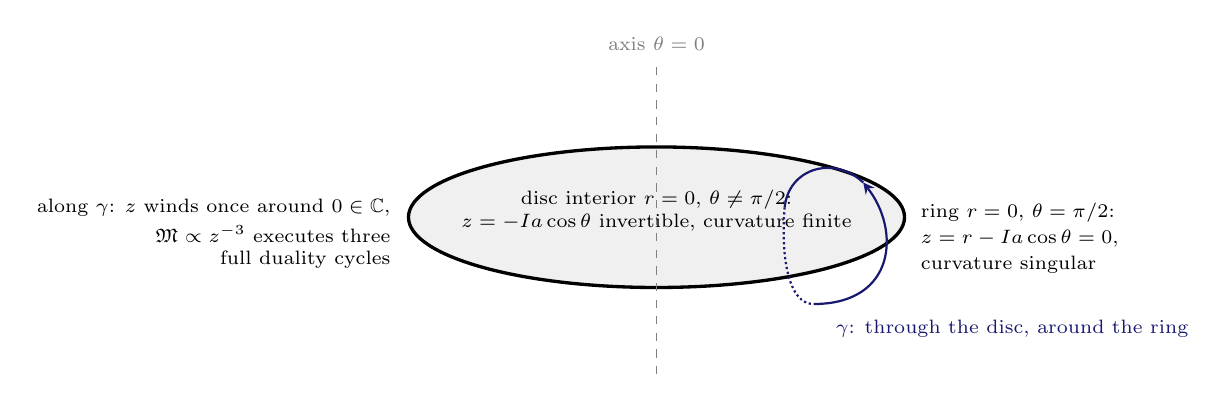
\begin{tikzpicture}[scale=1.05]
  % the disc r = 0 with the ring as its edge
  \fill[gray!12] (0,0) ellipse (3 and 0.85);
  \draw[very thick] (0,0) ellipse (3 and 0.85);
  % symmetry axis
  \draw[dashed, gray] (0,-1.9) -- (0,1.9);
  \node[gray, font=\scriptsize, anchor=south] at (0,1.9) {axis $\theta = 0$};
  % disc label
  \node[font=\scriptsize, align=center] at (0,0.08)
    {disc interior $r = 0$, $\theta \neq \pi/2$:\\ $z = -Ia\cos\theta$ invertible, curvature finite};
  % ring labels
  \node[font=\scriptsize, anchor=west] at (3.08,-0.25)
    {\shortstack[l]{ring $r = 0$, $\theta = \pi/2$:\\ $z = r - Ia\cos\theta = 0$,\\ curvature singular}};
  % the loop gamma through the disc, encircling the ring
  \draw[thick, MidnightBlue, -stealth]
    (1.9,-1.05) .. controls (2.9,-1.05) and (2.95,-0.15) .. (2.5,0.42);
  \draw[thick, MidnightBlue]
    (2.5,0.42) .. controls (2.15,0.75) and (1.6,0.6) .. (1.55,0.12);
  \draw[thick, MidnightBlue, densely dotted]
    (1.55,0.12) .. controls (1.5,-0.5) and (1.6,-1.05) .. (1.9,-1.05);
  \node[MidnightBlue, font=\scriptsize, anchor=west] at (2.05,-1.35)
    {$\gamma$: through the disc, around the ring};
  % winding annotation
  \node[font=\scriptsize, anchor=east, align=right] at (-3.1,-0.2)
    {\shortstack[r]{along $\gamma$: $z$ winds once around $0 \in \C$,\\
      $\mathfrak M \propto z^{-3}$ executes three\\ full duality cycles}};
\end{tikzpicture}
\caption{Where the framework's own criterion puts the Kerr singularity (Proposition \ref{prop:ring}). The scale of the curvature is $\mathfrak M = -M z^{-3}$ with $z = r - Ia\cos\theta$ valued in the commutative subalgebra $\R \oplus \R I \cong \C$ of $\Cl(1,3)$. The locus where $z$ fails to be invertible is $r^2 + a^2\cos^2\theta = 0$: exactly the ring, the boundary of the disc $r = 0$. On the disc interior $z = -Ia\cos\theta$ is invertible, so the curvature is finite there, purely pseudoscalar (dual): the regularity of the disc requires no further input. A loop $\gamma$ threading the disc and closing around the ring (dotted where it passes through the disc into the $r < 0$ sheet) winds $z$ once around $0 \in \C$, so the cubed pole winds the duality phase of the curvature three times: the monodromy of Remark \ref{rem:winding}, thrice the winding of the Killing spinor $\chi = z$ (Proposition \ref{prop:killing}), and the first invariant of Conjecture \ref{conj:monodromy}.}
\label{fig:ring}
\end{figure}

\subsection{The scale is the Killing spinor}\label{subsec:killing}

\begin{fact}[Imported: the Walker-Penrose Killing spinor]\label{fact:wp}
Every type-D vacuum admits a valence-two Killing spinor $\chi$, unique up to constant scale, whose square yields a conformal Killing-Yano tensor; for Kerr its scalar invariant is proportional to $r - ia\cos\theta$, and Carter's quartic constant of geodesic motion is the associated quadratic first integral; for type-D vacua the Weyl scalar and the spinor invariant are related by $\Psi_2 \propto \chi^{-3}$, the constant fixed by normalisation. \emph{Provenance:} the Killing spinor and the quadratic integral are Walker-Penrose \cite{WalkerPenrose1970}, the constant of motion Carter \cite{Carter1968}; the $\Psi_2 \propto \chi^{-3}$ relation is the standard type-$\{22\}$ statement descending from \cite{WalkerPenrose1970}, and for Kerr the corresponding statement about the framework's own scale $\mathfrak M$ is derived in Proposition \ref{prop:killing} from Fact \ref{fact:kerrcurv} and the Killing-spinor scalar above, with no appeal to this clause and none to the imported normalisation; the script checks that derivation.
\end{fact}

\begin{proposition}[The complex scale is the inverse cube of the Killing spinor]\label{prop:killing}
Identify the commutative subalgebra $\R \oplus \R I$ with $\C$ as in Proposition \ref{prop:ring}(1), matching $I$ with $i$ (an orientation choice, fixed once). Then the Kerr curvature scale of Fact \ref{fact:kerrcurv} is
\[
\mathfrak M \;=\; -M\,\chi^{-3}
\]
with $\chi = r - Ia\cos\theta$ the Killing-spinor scale of Fact \ref{fact:wp} in the same normalisation. Consequently: the framework's ``scalar-plus-pseudoscalar scale'', discovered in Proposition \ref{prop:shape} as the carrier of the entire approach to the singularity and complexified by rotation in Proposition \ref{prop:ring}, is a hidden twistorial object: the very spinor that generates Carter's constant and the hidden symmetries of the Kerr interior. And the duality monodromy of Remark \ref{rem:winding} is thrice the winding of the Killing spinor around the ring.
\end{proposition}

\begin{proof}
The content is an identification, and the proof is the comparison of the two displayed objects in one convention. By Fact \ref{fact:kerrcurv} and Proposition \ref{prop:ring} the scale is $\mathfrak M = -M(r - Ia\cos\theta)^{-3}$; by Fact \ref{fact:wp} the Killing-spinor scalar is $c\,(r - ia\cos\theta)$ for a nonzero constant $c$ fixed by normalising the spinor; choosing the normalisation $c = 1$ (which the constant-scale freedom of Fact \ref{fact:wp} permits) and matching $I \leftrightarrow i$ gives $\mathfrak M = -M\chi^{-3}$ exactly. What is \emph{not} conventional, and carries the content: (a) the power is three, so the winding statement of Remark \ref{rem:winding} is winding number three of $\chi$ itself; (b) the object on the left is constructed from curvature and the transport framework's invertibility criterion alone, with no reference to spinors, geodesics, or separability, while the object on the right generates Carter's constant; their identification is a nontrivial fact about where the framework's scale lies. The $\Psi_2 \propto \chi^{-3}$ clause of Fact \ref{fact:wp} is the spinor-calculus instance of this computation rather than an input to it: nothing above uses it, the derivation running on Fact \ref{fact:kerrcurv} and the Killing-spinor scalar alone, and $\mathfrak M$ is the type-D curvature scale that $\Psi_2$ names in the spinor conventions, equal to it up to the constant fixed by Fact \ref{fact:spectrum}.
\end{proof}

\begin{remark}[Points of contact with established physics, kept in view]\label{rem:kerrtouch}
As the series' practice requires, the points of contact are stated where they occur. The principal plane pair of Fact \ref{fact:kerrcurv} is the eigenplane structure of a type-D Weyl operator (Petrov); the Killing spinor is the standard generator of Kerr's hidden symmetry (Carter's constant, symmetry operators for wave equations); and the identification of Proposition \ref{prop:killing} places the framework's conformal scale inside twistor theory, whose systematic development for the series (ascended spinors, incidence, the palatial bridge) belongs to the twistor paper T9 \cite{ButlerT9}. Nothing in Parts one and two depended on these identifications; Part three's point is that the framework's internal objects coincide with them exactly.
\end{remark}

\subsection{The perturbed Cauchy horizon}\label{subsec:cauchy}

Exact Kerr was never the hard part of the test. Since Kerr is Ricci-flat, Theorem \ref{thm:parallel} applies verbatim on the whole vacuum region, inner horizons included: the parallel null tractor exists globally, and exact Kerr passes the covariance test outright. The physical question is what survives perturbation, because the Cauchy horizon is known to be unstable. The established results are imported with provenance and then read.

\begin{fact}[Imported: mass inflation and $C^0$ stability]\label{fact:cauchy}
(i) Infalling radiation is blueshifted without bound at the Kerr Cauchy horizon, generically driving unbounded growth of the quasi-local (Hawking) mass: mass inflation. (ii) For dynamical vacuum perturbations of Kerr initial data, the metric extends continuously ($C^0$) across the Cauchy horizon. (ii$'$) In spherical symmetry (the Einstein-Maxwell-scalar field system with two-ended asymptotically flat data), the metric extends continuously across the Cauchy horizon while, generically, the Christoffel symbols fail to be locally square-integrable: a weak null singularity. The same generic failure, with curvature blow-up, is the expected picture for the Kerr perturbations of (ii); it is stated there as a conjecture and is not proved. (iii) Tidal deformations of infalling observers remain finite through the weak null singularity. \emph{Provenance:} (i) Poisson-Israel \cite{PoissonIsrael1990}; (ii) Dafermos-Luk \cite{DafermosLuk2017}; (ii$'$) Luk-Oh \cite{LukOh2019a,LukOh2019b}; (iii) Ori \cite{Ori1991}.
\end{fact}

\begin{proposition}[The filtration at the Cauchy horizon, read from the literature]\label{prop:ordering}
In the framework's language, Fact \ref{fact:cauchy} yields three findings; each is a reading of the imported statements, and the one-step translation carrying each reading is proved below.
\begin{enumerate}
\item \emph{Obstruction type:} the degeneration at the perturbed Cauchy horizon is of type N (null kernel direction), in the degenerate-radical reading the series fixes at the Schwarzschild centre \cite[Prop.~3.1]{ButlerT5}, which extends T1's taxonomy \cite[Def.~3.1]{ButlerT1} to radical directions through \cite[Thm.~4.4, Cor.~4.5]{ButlerT4}: the same class as at the centre, realised on a null hypersurface rather than at a point.
\item \emph{Filtration by derivative level:} a $C^0$ metric determines a $C^0$ conformal class (pointwise multiplication by a positive function preserves continuity, and the class map $g \mapsto [g]$ is continuous), so point-level structure, metric and conformal alike, extends continuously across the Cauchy horizon, while connection-level structure, Levi-Civita and tractor alike (the tractor connection carries the Schouten tensor, two derivatives of $g$), generically fails: proved in spherical symmetry by Fact \ref{fact:cauchy}(ii$'$), expected for Kerr. The ordering is by derivative level; a strict separation of the conformal description from the metric one at fixed derivative level is not among the imports, and is exactly the open transport question of Section \ref{sec:scope}.
\item \emph{Filtration:} in a frame adapted to the horizon generators, the divergent curvature components are those of extreme boost weight, the top of the parabolic filtration attached to the null direction: the divergence occupies the nilpotent slots, as in every previous instance of the obstruction.
\end{enumerate}
\end{proposition}

\begin{proof}
(1) The degenerating direction is the null generator of the Cauchy horizon; the kernel of the degenerating metric data is spanned by a null vector, the type-N condition in the degenerate-radical reading imported above (T1's Definition 3.1 is stated for nondegenerate algebras; the extension to radical directions is T4's, routed as at the Schwarzschild centre through \cite[Prop.~3.1]{ButlerT5}). (2) The mathematical content is elementary and proved here: if $g_n \to g$ in $C^0$ with $g$ a continuous nondegenerate metric, then for any continuous positive $\omega$, $\omega g_n \to \omega g$ in $C^0$, so the conformal class of the $C^0$ extension is a $C^0$-extended conformal class; Fact \ref{fact:cauchy}(ii) supplies the $C^0$ metric extension for Kerr perturbations, and Fact \ref{fact:cauchy}(ii$'$) the generic failure at one derivative, proved in spherical symmetry and expected for Kerr. At connection level the two descriptions succeed or fail together: the tractor connection \eqref{eq:tractorconn} carries the Levi-Civita action and the Schouten tensor, first and second derivatives of $g$, so the generic failure of Fact \ref{fact:cauchy}(ii$'$) reaches it exactly where it reaches the metric connection; no separation between the descriptions is claimed, or available, from the imports. (3) is the boost-weight structure of weak null singularities as established in the works cited in Fact \ref{fact:cauchy}: the blow-up is in the transversal derivative components, which carry extreme weight under the boost fixing the horizon generator; we import the analytic statement and observe only that extreme boost weight is precisely the nilradical slot of the parabolic fixing the null direction (Proposition \ref{prop:flatstab}(3)).
\end{proof}

\begin{remark}[The conclusion, and two cautions]\label{rem:verdict}
Proposition \ref{prop:ordering}(2) is a filtration statement, and it is read as exactly that: survival at the perturbed Cauchy horizon is ordered by derivative level, with the divergence in the nilpotent slots, which is the structure the framework predicts. What the literature does not supply is a strict separation of the conformal from the metric description at fixed derivative level: the framework's central claim, that the ascended description persists where the metric one fails, therefore rests at the Cauchy horizon on the open transport question of successor problem (1), not on a finished theorem. The Kerr test is passed at the level the imports reach, and no further. Two cautions make the conclusion more precise, both recorded as scope. First, generic perturbations destroy type-D rigidity: the exact shape factorisations of Propositions \ref{prop:shape} and \ref{prop:ring} are properties of the exact family, and robust statements off it must be made at the level of the boost-weight filtration rather than the fixed operator $S$. Second, what the framework most needs, a quantitative transport theorem (convergence of tractor parallel transport along causal curves crossing the Cauchy horizon), needs integrability of the connection along such curves: a property strictly between the established $C^0$ metric extension and the $C^1$ statement whose generic failure is proved in spherical symmetry and expected for Kerr, and not currently available in either direction. It is the sharpest open problem the test leaves, and it is registered in Section \ref{sec:scope}.
\end{remark}

\section{Scope, and successor problems}\label{sec:scope}

\subsection*{What is proved, what is imported, what is conjectured}

\emph{Proved in this paper, at the standard of \cite{ButlerT1}:} the unipotent-ray proposition and the exact scale decoupling (Propositions \ref{prop:unipotent}, \ref{prop:shape}); the elementary tractor lemmas and the entire flat-model dictionary (Lemma \ref{lem:elementary}, Propositions \ref{prop:flatstab}, \ref{prop:flatstabnn}); the vacuum theorem, the $\Lambda$ theorem with its internal sign-fixing, and the stabiliser rotation (Theorems \ref{thm:parallel}, \ref{thm:lambda}, Lemma \ref{lem:signpin}, Proposition \ref{prop:stabiliser}); the Kasner lemmas with explicit rates (Lemmas \ref{lem:kasnerform}, \ref{lem:parallel}, \ref{lem:conn}); the boost-generation lemma (Lemma \ref{lem:gen}); the weighted limit theorem and its Schwarzschild-de Sitter extension (Theorems \ref{thm:weighted}, \ref{thm:sds}), with the boundary holonomy algebra in the values-level sense fixed by Definition \ref{def:blowup}; the transport-level convergence theorem along tangential curves for the whole admissible class and its Schwarzschild $\varphi$-line corollary with rate (Theorem \ref{thm:duhamel}, Corollary \ref{cor:phi}); the Kerr-Schild unipotency and complex-factorisation propositions (Propositions \ref{prop:kerrschild}, \ref{prop:ring}); and the elementary halves of Propositions \ref{prop:killing} and \ref{prop:ordering}.

\emph{Imported as Facts with provenance:} the GTG-Einstein equivalence and the two curvature computations (Facts \ref{fact:gtg}, \ref{fact:spectrum}, \ref{fact:kerrcurv}); the tractor connection (Fact \ref{fact:tractor}); the Kerr-Schild form (Fact \ref{fact:kerrschild}); the Walker-Penrose spinor (Fact \ref{fact:wp}); the Cauchy-horizon results (Fact \ref{fact:cauchy}). Each is used only through its stated content.

\emph{Scoped and open:} the weighted limit theorem's scope is the admissible (Einstein velocity-dominated) class of Definition \ref{def:blowup}, with the mixmaster delimiter of Remark \ref{rem:delimiter} marking the provable boundary; the duality-monodromy conjecture (Conjecture \ref{conj:monodromy}) is posed, not proved; and the limits of the Kerr conclusion are itemised in Remark \ref{rem:verdict}.

\subsection*{Successor problems}

Five problems are named for the series' open directions, in decreasing order of urgency for the programme. (1) \emph{The quantitative transport theorem at the Cauchy horizon:} establish or refute integrability of the tractor connection along causal curves crossing the perturbed Cauchy horizon; either outcome sharpens Proposition \ref{prop:ordering} into a statement about the completion itself. (2) \emph{The billiard-invariant weighted limit:} formulate and prove the analogue of Theorem \ref{thm:weighted} on the quotient by Kasner-axis dynamics, where the generic mixmaster approach lies; the admissibility integral of Definition \ref{def:blowup} says exactly what fails framewise. (3) \emph{The ring blow-up:} extend the wall theory of \cite{ButlerT4} to codimension two and prove or refute Conjecture \ref{conj:monodromy}; the winding number three of Proposition \ref{prop:killing} is the first invariant any such theory must reproduce. (4) \emph{Edge regularity in general:} for a general admissible metric, control the tangential derivatives of the error $E_{\tau}$ on compact sets of the exceptional set, which admissibility does not include; this is the only analysis left in the edge problem, since the transport-level comparison along all tangential curves of fixed Hubble-normalised length is Theorem \ref{thm:duhamel} for the whole admissible class and the tangential regularity holds at Schwarzschild by symmetry (Corollary \ref{cor:phi}). (5) \emph{Carter's constant inside GTG:} derive the quadratic first integral directly from the scale identification of Proposition \ref{prop:killing} within the gauge-theoretic formalism, completing the connection the identification begins. The weighted completion of the wall program in its generic-singularity extension depends on (2) and on (4); the density constant $\nu$ of the entropy paper is stated for Schwarzschild, inside the admissible class with constant exponents and no bounces, where (2) does not arise and (4) is closed, so what that prediction still waits on is the calibration of the count, not analysis here.

\section{Position in the series}\label{sec:position}

This paper is T6 of the series. It consumes four predecessors. From the primer T0 \cite{ButlerT0} it takes the working language of geometric algebra; from the root paper T1 \cite{ButlerT1} the zero-divisor taxonomy, the no-go theorem whose transvections reappear here as the nilradical of the frozen point's stabiliser, and the completion that fixes the ambient algebra $\Cl(2,4)$; from the sheaf paper T4 \cite{ButlerT4} the wall-level theory of degeneration whose codimension-two extension Conjecture \ref{conj:monodromy} names; and from the singularity paper T5 \cite{ButlerT5} the curvature computation imported as Fact \ref{fact:spectrum} and the six-step chain whose three geometric links this paper closes. It supplies, downstream: the Hawking paper T7 \cite{ButlerT7} imports the GTG equivalence and the vacuum theorem (Fact \ref{fact:gtg}, Theorem \ref{thm:parallel}); the entropy paper T8 \cite{ButlerT8} builds on the Kasner form of the interior (Lemma \ref{lem:kasnerform}), the weighted-limit results of Section \ref{sec:approach}, and the duality-monodromy conjecture (Conjecture \ref{conj:monodromy}); the twistor paper T9 \cite{ButlerT9} develops the flat-model dictionary of Section \ref{sec:tractor}, the vacuum and $\Lambda$ theorems, and the Killing-spinor identification (Proposition \ref{prop:killing}); and the dark-energy paper T10 \cite{ButlerT10} takes the frozen point, its norm $\Lambda/3$, and the parabolic-to-reductive stabiliser rotation (Theorems \ref{thm:parallel}, \ref{thm:lambda}, Proposition \ref{prop:stabiliser}) as its kinematic base.

\section{Machine verification}\label{sec:verification}

Every computational identity of Parts one and two, and every printed constant of Part three, is verified by the deposited script \verb|verify_T06.py| \cite{ButlerVerifyT06}, which imports the series' shared exact-arithmetic library \verb|GA.py| and runs in exact rational arithmetic, so every check is an identity, not an approximation, with the single exception of one CONTROL check in floating point (marked as such, on matrix exponentials, whose exact content is carried by the six identities beside it). Eighty-two checks pass: eighty-one exact checks and the CONTROL check, which needs \verb|numpy| and \verb|scipy|; when those cannot be imported the script prints an explicit SKIPPED line for it and the count is eighty-one, so a reader without them can still run every exact check. The coverage, by part. \emph{Part one:} the pseudoscalar algebra; the unipotent ray (Proposition \ref{prop:unipotent}: $P^2 = 0$ on the frame, the group law, the closed-form inverse, all Painlev\'e-Gullstrand metric entries at sample rational $\beta$ inside, at, and outside the horizon ($\beta = 1$ included), and the null roots $\lambda = -\beta \pm 1$); the shape operator (Proposition \ref{prop:shape}: the conjugation table, the spectrum $(-2,-2,1,1,1,1)$, $S^2 + S = 2$ as an operator identity on all six frame planes, the trace summed from the computed spectrum). \emph{Part two:} the flat model over $\mathbb{Q}$ (Proposition \ref{prop:flatstab}: the point embedding is null with the stated pairing, the stabiliser of the vector $\nInf$ has dimension exactly ten and of the ray eleven, computed as kernel ranks of the $15 \times 6$ action matrix by exact Gaussian elimination; the grading, Levi, and nilradical actions; two-step nilpotency of $\nInf \wedge w$ with square image in $\R\nInf$, and the exact translation exponential $e^{tN}X(x) = X(x - tw)$ at rational samples); the non-null stabilisers (Proposition \ref{prop:flatstabnn}: dimension ten and complement signatures $(1,4)$ and $(2,3)$ by exact congruence diagonalisation); the Schouten arithmetic of Lemma \ref{lem:elementary} and Theorem \ref{thm:lambda} as identities of rational functions in a formal $\Lambda$; and the algebraic part of the tractor connection \eqref{eq:tractorconn} as a $6 \times 6$ matrix: metric preservation (Lemma \ref{lem:elementary}(i)) with a flipped-sign control, $\nabla_a I_g = (0, -\Sch_{ab}, 0)$ and the null norm (Theorem \ref{thm:parallel}), and the parallelism of $(1, 0, \Lambda/6)$ with norm $\Lambda/3$ evaluated through the tractor metric, with a non-Einstein control (Theorem \ref{thm:lambda}), and the index order of the Schouten slot fixed on a non-symmetric sample. \emph{Part three, first half:} the Kasner exponent identities; for Section \ref{subsec:tangential}, the series $S(r) = 1 + \tfrac{3}{10}r + \tfrac{9}{56}r^2 + \cdots$, the expansion of $\tau\sigma_3$ with its three printed coefficients and the sign of every computed coefficient of $\delta$, the leading $\tfrac23\cot\theta\, r^{1/2}$ of the rotation coefficient $\varepsilon$ built from the $\tau$ series at a rational latitude, the rates in $\tau$ read off the leading exponents of $\delta$, $\varepsilon$ and $\tau$ against the constructed inversion $(3\tau/2)^{2/3} = r + O(r^2)$, and the Cauchy-Schwarz bound $\|H\| \le 1$ of Theorem \ref{thm:duhamel} at rational unit directions, attained at the Schwarzschild exponents (Definition \ref{def:blowup}), plus the floating-point control that the transport distance halves per quartering of $r$ at three latitudes while a fixed coordinate segment diverges (Corollary \ref{cor:phi}); the series $\tau(\rho)$, its $\tfrac23$-power inversion, and the Hubble-normalised rates, as exact truncated power series in $\rho = \sqrt r$ (the printed constants $-\tfrac13$, $-\tfrac{4}{15}$, $\tfrac23$, $-\tfrac{2}{15}$ are all checked, via a J.C.P.\ Miller recurrence for rational powers of unit series, promoted into \verb|GA.py| for the series' later use); the identification of the Kasner exponents with the computed boundary values of the rates, and the $R$-variable expansion extracted from those rates by exact division against $R(\rho)$, its constants matching the printed ones and its residual starting at $\rho^6$; the boost-generation lemma (Lemma \ref{lem:gen}: the commutator closure of the three boosts has dimension exactly six, contains all three rotations, and annihilates both null directions); and the Schwarzschild-de Sitter comparison (Theorem \ref{thm:sds}: the $\tau$-coefficients agree through order $\rho^8$ at two rational values of $\Lambda$, the first discrepancy is exactly $-\Lambda\rho^9/27$ and linear in $\Lambda$, and the rate constants are unchanged). \emph{Part three, second half:} Kerr-Schild unipotency ($P_k^2 = 0$, and the inverse-metric and metric identities $\hb(a)\cdot\hb(b) = a\cdot b + 2H(a\cdot k)(b\cdot k)$ and $\hb^{-1}(a)\cdot\hb^{-1}(b) = a\cdot b - 2H(a\cdot k)(b\cdot k)$ on all sixteen frame pairs at three values of $H$); the complex subalgebra as a field with exact inverses; the disc-interior scale $M I (a\cos\theta)^{-3}$, built from an independently computed inverse cube; the reduction at $a = 0$, where the real scale $-M/r^3$ returns Fact \ref{fact:spectrum}'s eigenvalues $+2M/r^3$ on the plane pair and $-M/r^3$ on the four mixed planes, with the opposite overall convention failing as a control; the complex eigenvalue table $2 : (-1)$ with the same $S$, now on complexified bivectors; and the Killing-spinor identity $\chi^3\,\mathfrak M = -M$, with $\mathfrak M$ built from an independently computed inverse cube and negative controls at exponents two and four. The script exits nonzero on any failure and prints one line per check, tagged by the statement it certifies.

\begin{thebibliography}{99}

\bibitem{ButlerT0}
L.~Butler,
\emph{An Introduction to Geometric Algebra: A Primer for the Transport Papers},
Transport Papers T0 (2026).

\bibitem{ButlerT1}
L.~Butler,
\emph{The Transport Principle: Total Division in Clifford Algebras via Minimal Completion},
Transport Papers T1 (2026).

\bibitem{ButlerT4}
L.~Butler,
\emph{Clifford Sheaves over Degenerate Metrics: Nilpotent Ideals, One-Sided Completion, and the Exceptional Algebra},
Transport Papers T4 (2026).

\bibitem{ButlerT5}
L.~Butler,
\emph{Division by Zero at the Gravitational Singularity: The Transport Principle Applied to the Black Hole, and the Information Paradox as a Category Error},
Transport Papers T5 (2026).

\bibitem{ButlerT7}
L.~Butler,
\emph{Hawking Radiation from the Ledger: State, Continuum, Lift, and the Finite-Ledger Seam},
Transport Papers T7 (2026).

\bibitem{ButlerT8}
L.~Butler,
\emph{Black-Hole Entropy and Scrambling: The Singularity Ledger and the No-Echo Prediction},
Transport Papers T8 (2026).

\bibitem{ButlerT9}
L.~Butler,
\emph{The Twistor Correspondence: Ascended Spinors, Incidence, and the Palatial Bridge},
Transport Papers T9 (2026).

\bibitem{ButlerT10}
L.~Butler,
\emph{Dark Energy and the Action of Gravity: MacDowell-Mansouri, the Frozen Point, and One Way to Grip},
Transport Papers T10 (2026).

\bibitem{LDG1998}
A.~Lasenby, C.~Doran and S.~Gull,
Gravity, gauge theories and geometric algebra,
\emph{Phil.\ Trans.\ R.\ Soc.\ Lond.\ A} \textbf{356} (1998), 487--582.

\bibitem{DoranLasenby2003}
C.~Doran and A.~Lasenby,
\emph{Geometric Algebra for Physicists},
Cambridge University Press (2003).

\bibitem{BEG1994}
T.~N.~Bailey, M.~G.~Eastwood and A.~R.~Gover,
Thomas's structure bundle for conformal, projective and related structures,
\emph{Rocky Mountain J.\ Math.} \textbf{24} (1994), 1191--1217.

\bibitem{CurryGover2018}
S.~N.~Curry and A.~R.~Gover,
An introduction to conformal geometry and tractor calculus, with a view towards analysis on manifolds,
in \emph{Asymptotic Analysis in General Relativity},
London Mathematical Society Lecture Note Series 443, Cambridge University Press (2018), 86--170.

\bibitem{Gover2010}
A.~R.~Gover,
Almost Einstein and Poincar\'e-Einstein manifolds in Riemannian signature,
\emph{J.\ Geom.\ Phys.} \textbf{60} (2010), 182--204.

\bibitem{ELS1972}
D.~Eardley, E.~Liang and R.~Sachs,
Velocity-dominated singularities in irrotational dust cosmologies,
\emph{J.\ Math.\ Phys.} \textbf{13} (1972), 99--107.

\bibitem{IsenbergMoncrief1990}
J.~Isenberg and V.~Moncrief,
Asymptotic behavior of the gravitational field and the nature of singularities in Gowdy spacetimes,
\emph{Ann.\ Phys.} \textbf{199} (1990), 84--122.

\bibitem{BKL1970}
V.~A.~Belinskii, I.~M.~Khalatnikov and E.~M.~Lifshitz,
Oscillatory approach to a singular point in the relativistic cosmology,
\emph{Adv.\ Phys.} \textbf{19} (1970), 525--573.

\bibitem{DHN2003}
T.~Damour, M.~Henneaux and H.~Nicolai,
Cosmological billiards,
\emph{Class.\ Quantum Grav.} \textbf{20} (2003), R145--R200.

\bibitem{KerrSchild1965}
R.~P.~Kerr and A.~Schild,
Some algebraically degenerate solutions of Einstein's gravitational field equations,
\emph{Proc.\ Symp.\ Appl.\ Math.} \textbf{17} (1965), 199--209.

\bibitem{WalkerPenrose1970}
M.~Walker and R.~Penrose,
On quadratic first integrals of the geodesic equations for type $\{22\}$ spacetimes,
\emph{Commun.\ Math.\ Phys.} \textbf{18} (1970), 265--274.

\bibitem{Carter1968}
B.~Carter,
Global structure of the Kerr family of gravitational fields,
\emph{Phys.\ Rev.} \textbf{174} (1968), 1559--1571.

\bibitem{PoissonIsrael1990}
E.~Poisson and W.~Israel,
Internal structure of black holes,
\emph{Phys.\ Rev.\ D} \textbf{41} (1990), 1796--1809.

\bibitem{Ori1991}
A.~Ori,
Inner structure of a charged black hole: an exact mass-inflation solution,
\emph{Phys.\ Rev.\ Lett.} \textbf{67} (1991), 789--792.

\bibitem{DafermosLuk2017}
M.~Dafermos and J.~Luk,
The interior of dynamical vacuum black holes I: the $C^0$-stability of the Kerr Cauchy horizon,
preprint, arXiv:1710.01722 (2017).

\bibitem{LukOh2019a}
J.~Luk and S.-J.~Oh,
Strong cosmic censorship in spherical symmetry for two-ended asymptotically flat initial data I. The interior of the black hole region,
\emph{Ann.\ of Math.\ (2)} \textbf{190} (2019), 1--111.

\bibitem{LukOh2019b}
J.~Luk and S.-J.~Oh,
Strong cosmic censorship in spherical symmetry for two-ended asymptotically flat initial data II. The exterior of the black hole region,
\emph{Ann.\ PDE} \textbf{5} (2019), Art.\ 6.

\bibitem{ButlerVerifyT06}
L.~Butler,
\emph{verify\_T06.py: exact-arithmetic verification of the computational identities of ``The Geometry of the Black-Hole Interior''},
Python script, deposited with this paper alongside the shared library GA.py (2026).

\end{thebibliography}

\end{document}
